\RequirePackage{atbegshi}
\documentclass[compress,aspectratio=169]{beamer} % aspectratio=169
%\usepackage[svgnames]{xcolor}

%	%	%	%	%	%	%	%	%	%	%	%	%	%	%
% 						MY PACKAGES 
%	%	%	%	%	%	%	%	%	%	%	%	%	%	%
\usepackage{graphicx}				% Use pdf, png, jpg, or eps with pdflatex; use eps in DVI mode

\usepackage[export]{adjustbox}

\usepackage{amssymb}
\usepackage{amsmath}	
%\usepackage{tipx}
%\usepackage{tikz}
%\usetikzlibrary{arrows,shapes,decorations.pathmorphing,backgrounds,positioning,fit,petri}
\usepackage{rotating}
\usepackage{scalerel} % for inline images
\usepackage{import}
%\usepackage{times}
\usepackage{array}
\usepackage{tabularx}
%\usepackage{booktabs}
\usepackage{textcomp}
\usepackage{caption}
\usepackage{float}
%\usepackage{setspace} 			% \doublespacing \singlespacing \onehalfspacing	%doble espacio
%\label{x:y}													%ocupar para autoref.
%\autoref{x:y}												%ocupar para autoref.
%\usepackage{nopageno}			%desactivar para p�ginas
\usepackage{pifont}
%\usepackage{color,xcolor,ucs}
%\usepackage{marvosym} %faces

\usepackage{hyperref}
\usepackage{multirow}

\usepackage{listings}
\usepackage{color}
\definecolor{dkgreen}{rgb}{0,0.6,0}
\definecolor{gray}{rgb}{0.5,0.5,0.5}
\definecolor{mauve}{rgb}{0.58,0,0.82}
\lstset{ %
  language=R,                     % the language of the code
  basicstyle=\TINY,      			% the size of the fonts that are used for the code
  numbers=left,                   % where to put the line-numbers
  numberstyle=\tiny\color{gray},  % the style that is used for the line-numbers
  stepnumber=1,                   % the step between two line-numbers. If it's 1, each line
                                  % will be numbered
  numbersep=5pt,                  % how far the line-numbers are from the code
  backgroundcolor=\color{white},  % choose the background color. You must add \usepackage{color}
  showspaces=false,               % show spaces adding particular underscores
  showstringspaces=false,         % underline spaces within strings
  showtabs=false,                 % show tabs within strings adding particular underscores
  frame=single,                   % adds a frame around the code
  rulecolor=\color{black},        % if not set, the frame-color may be changed on line-breaks within not-black text (e.g. commens (green here))
  tabsize=1,                      % sets default tabsize to 2 spaces
  captionpos=b,                   % sets the caption-position to bottom
  breaklines=true,                % sets automatic line breaking
  breakatwhitespace=false,        % sets if automatic breaks should only happen at whitespace
  title=\lstname,                 % show the filename of files included with \lstinputlisting;
                                  % also try caption instead of title
  keywordstyle=\color{blue},      % keyword style
  commentstyle=\color{dkgreen},   % comment style
  stringstyle=\color{mauve},      % string literal style
  escapeinside={\%*}{*)},         % if you want to add a comment within your code
  morekeywords={*,...}            % if you want to add more keywords to the set
} 

%	%	%	%	%	%	%	%	%	%	%	%	%	%	%
% 					PACKAGE CUSTOMIZATION
%	%	%	%	%	%	%	%	%	%	%	%	%	%	%

% GENERAL CUSTOMIZATION
\usepackage[math]{iwona}% font
\usetheme{Singapore}	% template I should use
%\usetheme{Szeged}	% alternative template
\usecolortheme{rose}	% color template
\makeatletter			% to show subsection/section title (1/3)
\beamer@theme@subsectiontrue % to show subsection/section title (2/3)
\makeatother			% to show subsection/section title (3/3)



% THIS BELOW IS TO MAKE NAVIGATION DOTS MARKED DURING PRESENTATION
\makeatletter
\def\slideentry#1#2#3#4#5#6{%
  %section number, subsection number, slide number, first/last frame, page number, part number
  \ifnum#6=\c@part\ifnum#2>0\ifnum#3>0%
    \ifbeamer@compress%
      \advance\beamer@xpos by1\relax%
    \else%
      \beamer@xpos=#3\relax%
      \beamer@ypos=#2\relax%
    \fi%
  \hbox to 0pt{%
    \beamer@tempdim=-\beamer@vboxoffset%
    \advance\beamer@tempdim by-\beamer@boxsize%
    \multiply\beamer@tempdim by\beamer@ypos%
    \advance\beamer@tempdim by -.05cm%
    \raise\beamer@tempdim\hbox{%
      \beamer@tempdim=\beamer@boxsize%
      \multiply\beamer@tempdim by\beamer@xpos%
      \advance\beamer@tempdim by -\beamer@boxsize%
      \advance\beamer@tempdim by 1pt%
      \kern\beamer@tempdim
      \global\beamer@section@min@dim\beamer@tempdim
      \hbox{\beamer@link(#4){%
          \usebeamerfont{mini frame}%
          \ifnum\c@section>#1%
            %\usebeamercolor[fg]{mini frame}%
            %\usebeamertemplate{mini frame}%
            \usebeamercolor{mini frame}%
            \usebeamertemplate{mini frame in other subsection}%
          \else%
            \ifnum\c@section=#1%
              \ifnum\c@subsection>#2%
                \usebeamercolor[fg]{mini frame}%
                \usebeamertemplate{mini frame}%
              \else%
                \ifnum\c@subsection=#2%
                  \usebeamercolor[fg]{mini frame}%
                  \ifnum\c@subsectionslide<#3%
                    \usebeamertemplate{mini frame in current subsection}%
                  \else%
                    \usebeamertemplate{mini frame}%
                  \fi%
                \else%
                  \usebeamercolor{mini frame}%
                  \usebeamertemplate{mini frame in other subsection}%
                \fi%
              \fi%
            \else%
              \usebeamercolor{mini frame}%
              \usebeamertemplate{mini frame in other subsection}%
            \fi%
          \fi%
        }}}\hskip-10cm plus 1fil%
  }\fi\fi%
  \else%
  \fakeslideentry{#1}{#2}{#3}{#4}{#5}{#6}%
  \fi\ignorespaces
  }
\makeatother

%	%	%	%	%	%	%	%	%	%	%	%	%	%	%
% 			To show the TITLE at the Bottom of each slide
%	%	%	%	%	%	%	%	%	%	%	%	%	%	%

\beamertemplatenavigationsymbolsempty 
\makeatletter
\setbeamertemplate{footline}
{
\leavevmode%
\hbox{%
\begin{beamercolorbox}[wd=1\paperwidth,ht=2.25ex,dp=2ex,center]{title in head/foot}%
\usebeamerfont{title in head/foot}\insertshorttitle
\end{beamercolorbox}%
\begin{beamercolorbox}[wd=1
\paperwidth,ht=2.25ex,dp=2ex,center]{date in head/foot}%
\end{beamercolorbox}}%
}
\makeatother



% to switch off navigation bullets
%% using \miniframeson or \miniframesoff
\makeatletter
\let\beamer@writeslidentry@miniframeson=\beamer@writeslidentry
\def\beamer@writeslidentry@miniframesoff{%
  \expandafter\beamer@ifempty\expandafter{\beamer@framestartpage}{}% does not happen normally
  {%else
    % removed \addtocontents commands
    \clearpage\beamer@notesactions%
  }
}
\newcommand*{\miniframeson}{\let\beamer@writeslidentry=\beamer@writeslidentry@miniframeson}
\newcommand*{\miniframesoff}{\let\beamer@writeslidentry=\beamer@writeslidentry@miniframesoff}
\makeatother

% Image full size: use 
%%\begin{frame}
  %%\fullsizegraphic{monogram.jpg}
%%\end{frame}
\newcommand<>{\fullsizegraphic}[1]{
  \begin{textblock*}{0cm}(-1cm,-3.78cm)
  \includegraphics[width=\paperwidth]{#1}
  \end{textblock*}
}


% hyperlinks
\hypersetup{colorlinks,
            urlcolor=[rgb]{0.01, 0.28, 1.0},
            linkcolor=[rgb]{0.01, 0.28, 1.0}}


%	%	%	%	%	%	%	%	%	%	%	%	%	%	%
% 					DOCUMENT ID
%	%	%	%	%	%	%	%	%	%	%	%	%	%	%

\title{\href{https://github.com/hbahamonde/Earthquake_Paper/raw/master/Bahamonde_Earthquake_Paper.pdf}{\input{/Users/hectorbahamonde/RU/Dissertation/Papers/Earthquake_Paper/title.txt}\unskip}}
\author{Hector Bahamonde $\bullet$ Assistant Professor $\bullet$ Universidad de O$'$Higgins}
\date{\today}

%to to see shadows of previous blocks
%\setbeamercovered{dynamic}


\begin{document}



%	%	%	%	%	%	%	%	%	%	%	%	%	%	%
% 					CONTENT
%	%	%	%	%	%	%	%	%	%	%	%	%	%	%

%% title frame

\begin{frame}[label = cover]
\titlepage
\end{frame}



\section{Introduction}

%section{Outline}
\subsection{Preliminaries}

\miniframeson
\begin{frame}\frametitle{Overview}

	\begin{itemize}
		\item[{\tiny [{\bf Origins}]}] Most theories emphasize how important fiscal development is for state consolidation. {\color{red}However}, the {\bf origins} of fiscal development are less clear.

		\item[{\tiny [{\bf Measurement}]}] Most theories provide {\bf historical} explanations for state consolidation, {\color{red}yet}, they lack of a {\bf historical} measurement capable of capturing levels of state capacities overtime.

		\item I find that these two gaps represent important {\bf theoretical} and {\bf empirical}  {\color{red}\bf deficits}.
	\end{itemize}

\end{frame}


\miniframesoff
\begin{frame}\frametitle{Taxation and State Capacities}

{\bf Convince you}:

\begin{enumerate}
	\item Higher levels of sectoral competition promoted the implementation of the income tax.\pause
	\item The income tax fostered higher levels of state consolidation overtime.\pause
	\item Earthquake death-tolls are good proxies to measure state capacities.
\end{enumerate}

\end{frame}


\subsection{Motivation}





\miniframeson
\begin{frame}\frametitle{Why Earthquakes?}

\begin{itemize}
	\item[] The {\bf capacity} of the state to {\bf enforce} quake-sensitive {\bf building codes} throughout the territory, is a {\bf {\color{red}reflection}} of its {\bf overall} state-capacities.
\end{itemize}

	\vspace{-0.2cm}
		
		\begin{figure}[H]
		\hspace{-7mm}\frame{\includegraphics[scale=0.33]{/Users/hectorbahamonde/RU/Dissertation/Presentation/Resources/quake_map.jpg}}
		\end{figure}
	
\end{frame}


\miniframesoff
\begin{frame}\frametitle{Why Earthquakes?}

\begin{itemize}
	\item[] Earthquakes are {\bf exogenous} to regime type, levels of political/economic development, and other sources of variation.
\end{itemize}

	\vspace{-0.2cm}
		
		\begin{figure}[H]
		\hspace{-7mm}\frame{\includegraphics[scale=0.33]{/Users/hectorbahamonde/RU/Dissertation/Presentation/Resources/quake_map.jpg}}
		\end{figure}
	
\end{frame}


\miniframesoff
\begin{frame}\frametitle{Earthquakes and States Capacity}

	\vspace{-0.8cm}
	\begin{columns}

	\column{0.5\textwidth}
		\begin{figure}[H]
		\caption*{{\tiny {\color{red}{\bf 2010 Haiti: 7M, 100,000 casualties}\\\underline{Government Palace}}}}
		\hspace{-5mm}\frame{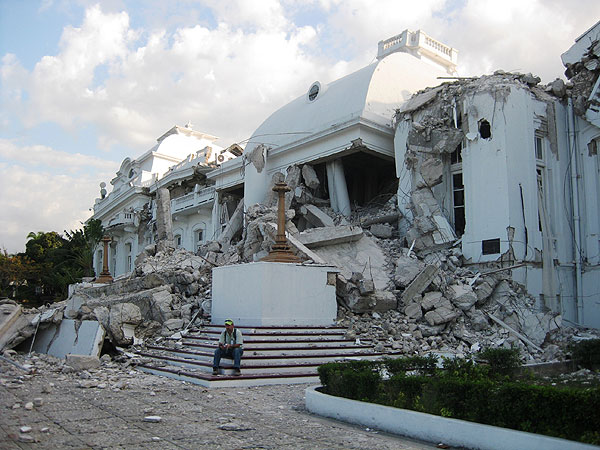
\includegraphics[scale=0.27]{/Users/hectorbahamonde/RU/Dissertation/Papers/Earthquake_Paper/Resources/haiti_quake}}
		\end{figure}

	\column{0.5\textwidth}
		
		\begin{figure}[H]
		\caption*{{\tiny {\color{black!30!green}{\bf 2010 Chile: 8.8M, 525 casualties}\\{\color{white}One of the {\bf few} buildings that actually collapsed}}}}
		\hspace{-7mm}\frame{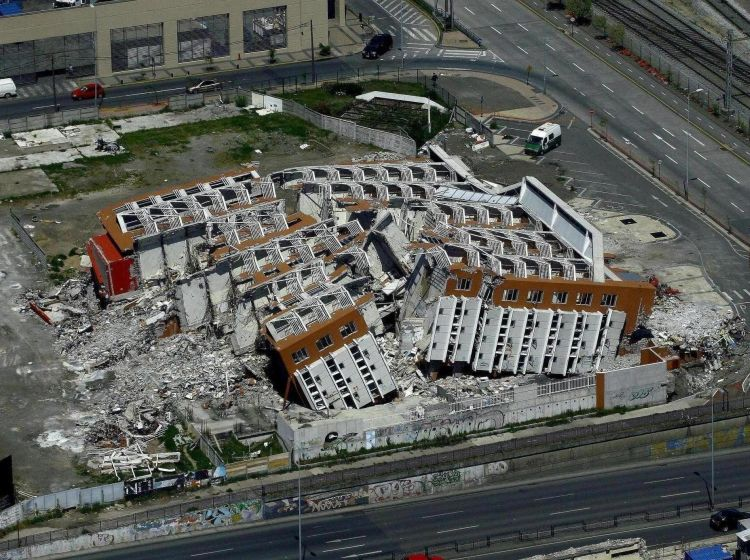
\includegraphics[scale=0.2]{/Users/hectorbahamonde/RU/Dissertation/Papers/Earthquake_Paper/Resources/alto_rio_quake}}
		\end{figure}
	
	\end{columns}

\begin{itemize}
	\pause\item[] {\color{black!30!green}{\bf Intuition}: Chile has higher levels of ``state capacity.''}
\end{itemize}

\end{frame}



\miniframesoff
\begin{frame}\frametitle{The Importance of Building Codes}

\begin{itemize}
	\item[] There exists a {\bf popular} consensus on that {\bf building codes} \emph{do} reduce death tolls. 
\end{itemize}
\vspace{-0.7cm}
	\begin{columns}

	\column{0.5\textwidth}
	
		\begin{figure}[H]
		\vspace{1mm}\frame{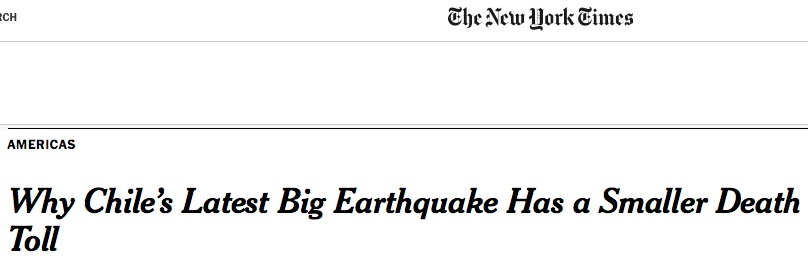
\includegraphics[scale=0.2]{/Users/hectorbahamonde/RU/Dissertation/Papers/Earthquake_Paper/Resources/nyt_quake}}
		\end{figure}


		\begin{figure}[H]
		\vspace{1mm}\frame{
\includegraphics[scale=0.2]{/Users/hectorbahamonde/RU/Dissertation/Papers/Earthquake_Paper/Resources/mexico_nyt}}
		\end{figure}

	\column{0.5\textwidth}
		
		\begin{figure}[H]
		\vspace{15mm}\hspace{-30mm}\frame{
\includegraphics[scale=0.19]{/Users/hectorbahamonde/RU/Dissertation/Papers/Earthquake_Paper/Resources/cnn_quake}}
		\end{figure}
	
	\end{columns}

\end{frame}





\section{Theory}


\subsection{Dual Economy}
\miniframeson
\begin{frame}\frametitle{Dual Political Economy and Taxation}
	
	\begin{itemize}
		

    \item \emph{``Lewis model:''} Industrialists and agriculturalists are in permanent {\bf {\color{red}conflict}}.\pause\; I {\color{red}extrapolate this conflict to politics}:\pause

            \begin{itemize}

                \item[] There are different {\color{red}sectoral preferences towards income taxation}, and consequently, {\bf state centralization}\pause:

                 %\item Since taxation {\color{red}affects} landowners and industrialists in {\color{red}different} ways, both sectors have different preferences towards state centralization.\pause

              \begin{enumerate}
                \item[{\color{red}[Agr]}] Since {\color{red}land fixity} increases the risk premium of the landed elite's main asset, landowners systematically {\color{red}resist} taxation.\pause

                \item[{\color{black!30!green}[Ind]}] As capital can be {\color{black!30!green}reinvested in nontaxable sectors}, industrialists' preferences toward taxation are more {\color{black!30!green}elastic}.
              \end{enumerate}


           \end{itemize}




	\end{itemize}

\end{frame}






\subsection{Fiscal Sociology}



% why income tax
\miniframeson
\begin{frame}\frametitle{Taxation and State Capacities}

	\begin{itemize}
		\item \emph{``Fiscal sociology:''} Income taxation offers a theory of state formation, and state centralization.\pause

		\item Monitoring private incomes, and converting them into {\color{red}public property}, \emph{fosters} state development:\pause

			\begin{enumerate}
				\item {\color{red}\emph{Indirect} taxes are {\bf easier} to collect}: ex., collect them at ports. \hyperlink{why_not_indirect_taxes}{\beamerbutton{appendix}}\pause
				\item {\color{black!30!green}\emph{Direct}} taxes (ex., income taxes)  require the {\bf {\color{red}deployment}} of tax collectors throughout the entire territory, increasing state presence.\pause
			\end{enumerate}

		\item {\bf ``Technology Adoption,'' ``Learning-By-Doing,'' \& ``Spillover Effects'' literatures}: Income taxation generated positive {\bf spillover effects} for state-making, rising {\bf economies of scale} of the {\bf operational efficiencies} of the bureaucracy.\

	\end{itemize}

\end{frame}






% p.3
\section{Argument}

%\miniframesoff
%\begin{frame}[plain,c]
%	\begin{center}
%	\vspace{5mm}
%	\Huge Did the implementation of the income tax in Chile increase state capacities over time? \\ \pause\;If so, how can those be measured?
%	\end{center}
%\end{frame}



%\miniframesoff
%\begin{frame}[plain,c]%\frametitle{Research Question}
%\begin{center}
%	\Huge{Use a novel hand-collected longitudinal {\bf dataset on earthquake death tolls} to proxy for the \emph{capacity} of the state to enforce building codes}
%\end{center}
%\end{frame}


%\miniframesoff
%\begin{frame}[plain,c]%\frametitle{Research Question}
%\begin{center}
%	\Huge{{\bf State capacities increase overtime upon the implementation of the income tax}}
%\end{center}
%\end{frame}













%\miniframesoff
%\begin{frame}\frametitle{Why Earthquakes?}
%
%\begin{itemize}
%	\item[] Importantly, enforcing these codes requires agreements with the subnational level. Subnational elites might not be interested in applying norms designed in the capital.
%\end{itemize}
%
%		
%		\begin{figure}[H]
%		%\vspace{20mm}\hspace{-30mm}
%		\frame{\includegraphics[scale=0.39]{/Users/hectorbahamonde/RU/Dissertation/Presentation/Resources/Montt_quake}}
%		\end{figure}
%	
%
%\end{frame}


%\subsection{Subnational Rationale}
%
%\miniframeson
%\begin{frame}\frametitle{Thinking Subnationally}
%	\begin{itemize}
%		
%		\item[] Since death tolls are a function of how well/bad building codes are enforced by the state throughout the {\bf territory}, adopting a {\bf subnational} approach seems more appropriate.
%
%		\begin{figure}[H]
		%\vspace{0.3cm}
%		\hspace{-8mm}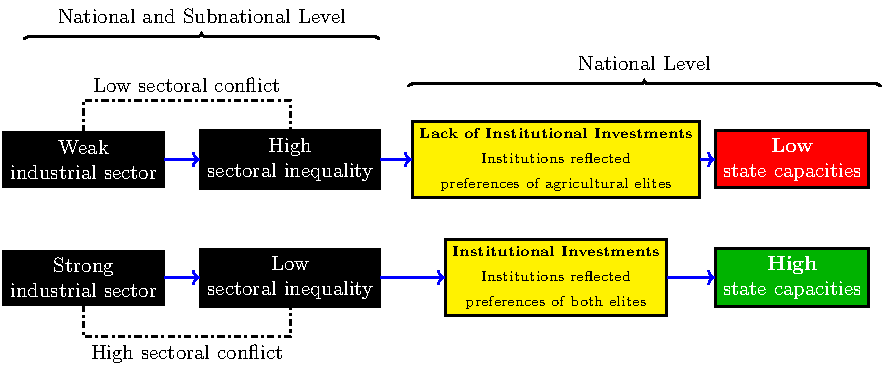
\includegraphics[scale=0.7]{/Users/hectorbahamonde/RU/Dissertation/Papers/Earthquake_Paper/causal_path}
%		\end{figure}

%	\end{itemize}
%\end{frame}

\subsection{Argument}

\miniframeson
\begin{frame}\frametitle{Argument (I)}
	\begin{itemize}
		
		\item[] The emergence of a {\color{red}strong industrial class}, accelerated the {\color{red}implementation of the income tax}. {\color{white}In turn, income taxation fostered {\color{white}state-capacities} overtime.}

		\begin{figure}[H]
		\vspace{10mm}\hspace{-8mm}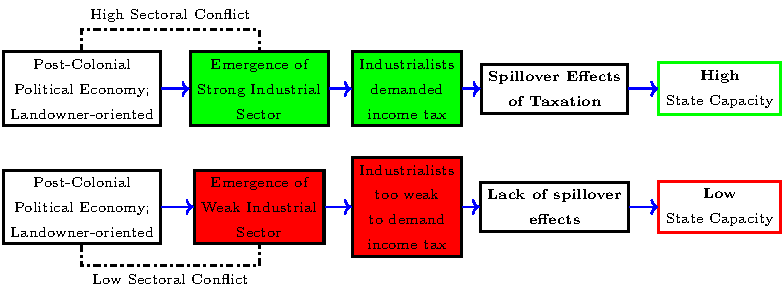
\includegraphics[scale=0.7]{/Users/hectorbahamonde/RU/Dissertation/Papers/Earthquake_Paper/Presentation/causal_path_1.pdf}
		\end{figure}

	\end{itemize}
\end{frame}


\miniframesoff
\begin{frame}\frametitle{Argument (II)}
  \begin{itemize}
    
    \item[] The emergence of a {\color{black}strong industrial class}, accelerated the implementation of the {\color{red}income tax}. {\color{black}In turn, income taxation fostered {\color{red}state-capacities} overtime.}

    \begin{figure}[H]
    \vspace{10mm}\hspace{-8mm}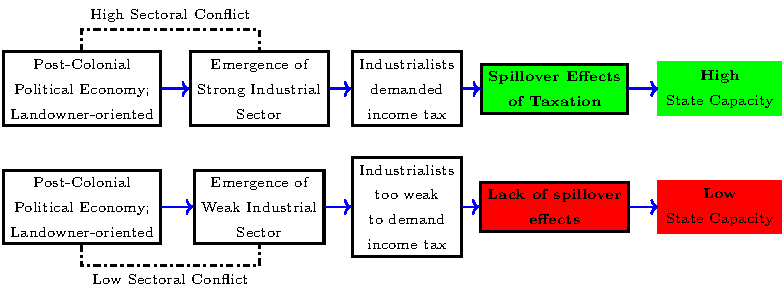
\includegraphics[scale=0.7]{/Users/hectorbahamonde/RU/Dissertation/Papers/Earthquake_Paper/Presentation/causal_path_2.pdf}
    \end{figure}

  \end{itemize}
\end{frame}


\miniframesoff
\begin{frame}\frametitle{Conceptualizing Sectoral Contestation}
  \begin{itemize}
    
    \item[] The {\color{red} post-colonial political economy} was ruled by {\color{red} agricultural} political incumbents. {\color{white}Consequently, the emergence of an industrial elite, posited credible threats to the post-colonial \emph{status quo}.}


    \begin{figure}[H]
    \vspace{5mm}\hspace{-8mm}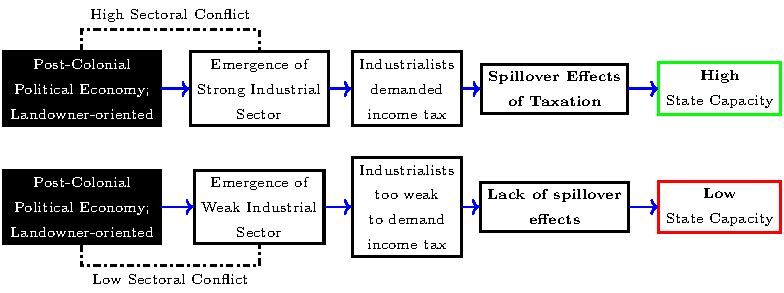
\includegraphics[scale=0.7]{/Users/hectorbahamonde/RU/Dissertation/Papers/Earthquake_Paper/Presentation/causal_path_3.pdf}
    \end{figure}

  \end{itemize}
\end{frame}


\miniframesoff
\begin{frame}\frametitle{Conceptualizing Sectoral Contestation}
  \begin{itemize}
    
    \item[] The post-colonial political economy was ruled by {\color{red} agricultural political incumbents}. {\color{black}Consequently, the emergence of an {\color{red} industrial} elite, posited {\color{red} credible threats} to the post-colonial \emph{status quo}.}


    \begin{figure}[H]
    \vspace{5mm}\hspace{-8mm}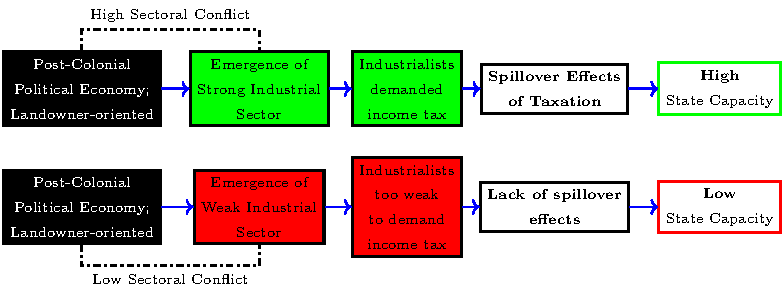
\includegraphics[scale=0.7]{/Users/hectorbahamonde/RU/Dissertation/Papers/Earthquake_Paper/Presentation/causal_path_4.pdf}
    \end{figure}

  \end{itemize}
\end{frame}



\miniframesoff
\begin{frame}\frametitle{Conceptualizing Sectoral Contestation}
  \begin{itemize}
    
    \item[] The sectoral threats had to do with the {\bf emergence} of a class---\emph{industrialists}---that were more {\color{red}sympathetic} to the idea of implementing an income tax law.


    \begin{figure}[H]
    \vspace{6mm}\hspace{-8mm}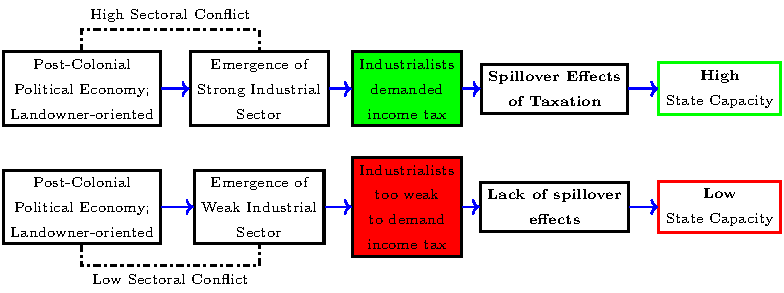
\includegraphics[scale=0.7]{/Users/hectorbahamonde/RU/Dissertation/Papers/Earthquake_Paper/Presentation/causal_path_5.pdf}
    \end{figure}

  \end{itemize}
\end{frame}


\subsection{Historical Evidence, and Mechanisms}
\miniframeson
\begin{frame}\frametitle{{\large Chilean Case Study}}
	\begin{itemize}

		\item Industrial elites were {\bf better off} paying the income tax rather than {\color{red}imposing higher tariffs}\pause---industrial class was highly \emph{dependent on imported capital}.\pause

   		\item In exchange of being income taxed, industrialists demanded public goods delivered at the local level (bridges and ports).

		%\item Activities such as {\bf deployment} of tax collectors to inspect accounting books and to supervise monetary transfers increased the {\color{red}density of state presence overtime.}

	\end{itemize}
\end{frame}


%\subsection{Alternative}
%\begin{frame}\frametitle{Counterfactual}
%	\begin{itemize}
%		
%		\item[] {\bf Persistences of colonial institutions}: post-colonial institutions would have {\color{red}reproduced} the {\color{red}hegemony} of agricultural elites (the ones that opposed income taxation).
%
%
%		\begin{figure}[H]
%		\frame{\includegraphics[scale=13.5]{/Users/hectorbahamonde/RU/Dissertation/Presentation/Resources/Baile_del_Santiago_antiguo}}\caption*{{\tiny `Baile del Santiago Antiguo.' Pedro Subercaseaux Err\'azuriz (1917).}}
%		\label{fig:baile}
%		\end{figure}
%		
%	\end{itemize}
%\end{frame}







\section{Econometrics}

\miniframeson
\subsection{Preliminaries}

\begin{frame}\frametitle{The Theory Should Pass Two Tests}
	
	\begin{enumerate}
		\item The income tax law should be {\bf implemented {\color{red}earlier}} under scenarios of {\color{red}\emph{high} sectoral contestation}.\pause\\{\footnotesize [\emph{rapid} industrial expansion]}\pause

		\item Implementation of the {\color{red}income tax} should produce {\color{red}\emph{higher} state-capacity}.\pause\\{\footnotesize [\emph{lower} death tolls overtime]}
	\end{enumerate}

\end{frame}


\subsection{Technical Details: Duration Models}

\miniframeson
\begin{frame}\frametitle{Early and Late Income-Tax Implementers}

        \begin{enumerate}
          \item[] {\bf Cox Model}. Sectoral outputs (\href{http://moxlad-staging.herokuapp.com/home/en?}{MOxLAD dataset}) to investigate the sectoral contribution to the {\color{red}timing} of the implementation of the income tax in 9 Latin American countries.\pause

          \item[] 
            \begin{equation*}\label{cox:eq}
              {\footnotesize h_{i}(t) = exp(\beta_{1}\text{Industrial Growth}_{i,t} + \beta_{2}\text{Agricultural Growth}_{i,t} + \beta_{3}\text{Total Population}_{i,t})h_{0}(t)}
            \end{equation*}
        \end{enumerate} 
  \hyperlink{duration_models}{\beamerbutton{reg table}}

\end{frame}

\miniframesoff
\begin{frame}\frametitle{Early and Late Income-Tax Implementers}

        \begin{enumerate}
          \item[] {\bf Cox Model}. Sectoral outputs (\href{http://moxlad-staging.herokuapp.com/home/en?}{MOxLAD dataset}) to investigate the sectoral contribution of the {\color{red}timing}  of the implementation of the income tax in 9 Latin American countries.

          \item[] 
            \begin{equation*}\label{cox:eq}
              {\footnotesize h_{i}(t) = exp(\beta_{1}\text{{\color{black!30!green}Industrial Growth}}_{i,t} + \beta_{2}\text{Agricultural Growth}_{i,t} + \beta_{3}\text{Total Population}_{i,t})h_{0}(t)}
            \end{equation*}
        \end{enumerate} 

  \hyperlink{duration_models}{\beamerbutton{reg table}}

\end{frame}


\begin{frame}\frametitle{Early and Late Income-Tax Implementers}

        \begin{enumerate}
          \item[] {\bf Cox Model}. Sectoral outputs (\href{http://moxlad-staging.herokuapp.com/home/en?}{MOxLAD dataset}) to investigate the sectoral contribution of the {\color{red}timing}  of the implementation of the income tax in 9 Latin American countries.

          \item[] 
            \begin{equation*}\label{cox:eq}
              {\footnotesize h_{i}(t) = exp(\beta_{1}\text{Industrial Growth}_{i,t} + \beta_{2}\text{{\color{red}Agricultural Growth}}_{i,t} + \beta_{3}\text{Total Population}_{i,t})h_{0}(t)}
            \end{equation*}
        \end{enumerate} 
  \hyperlink{duration_models}{\beamerbutton{reg table}}

\end{frame}



\miniframesoff
\begin{frame}[plain]\frametitle{Mexico: 1925}
     \begin{figure}[H]
  %   \vspace{4mm}
  %   \hspace{-7.5mm}
  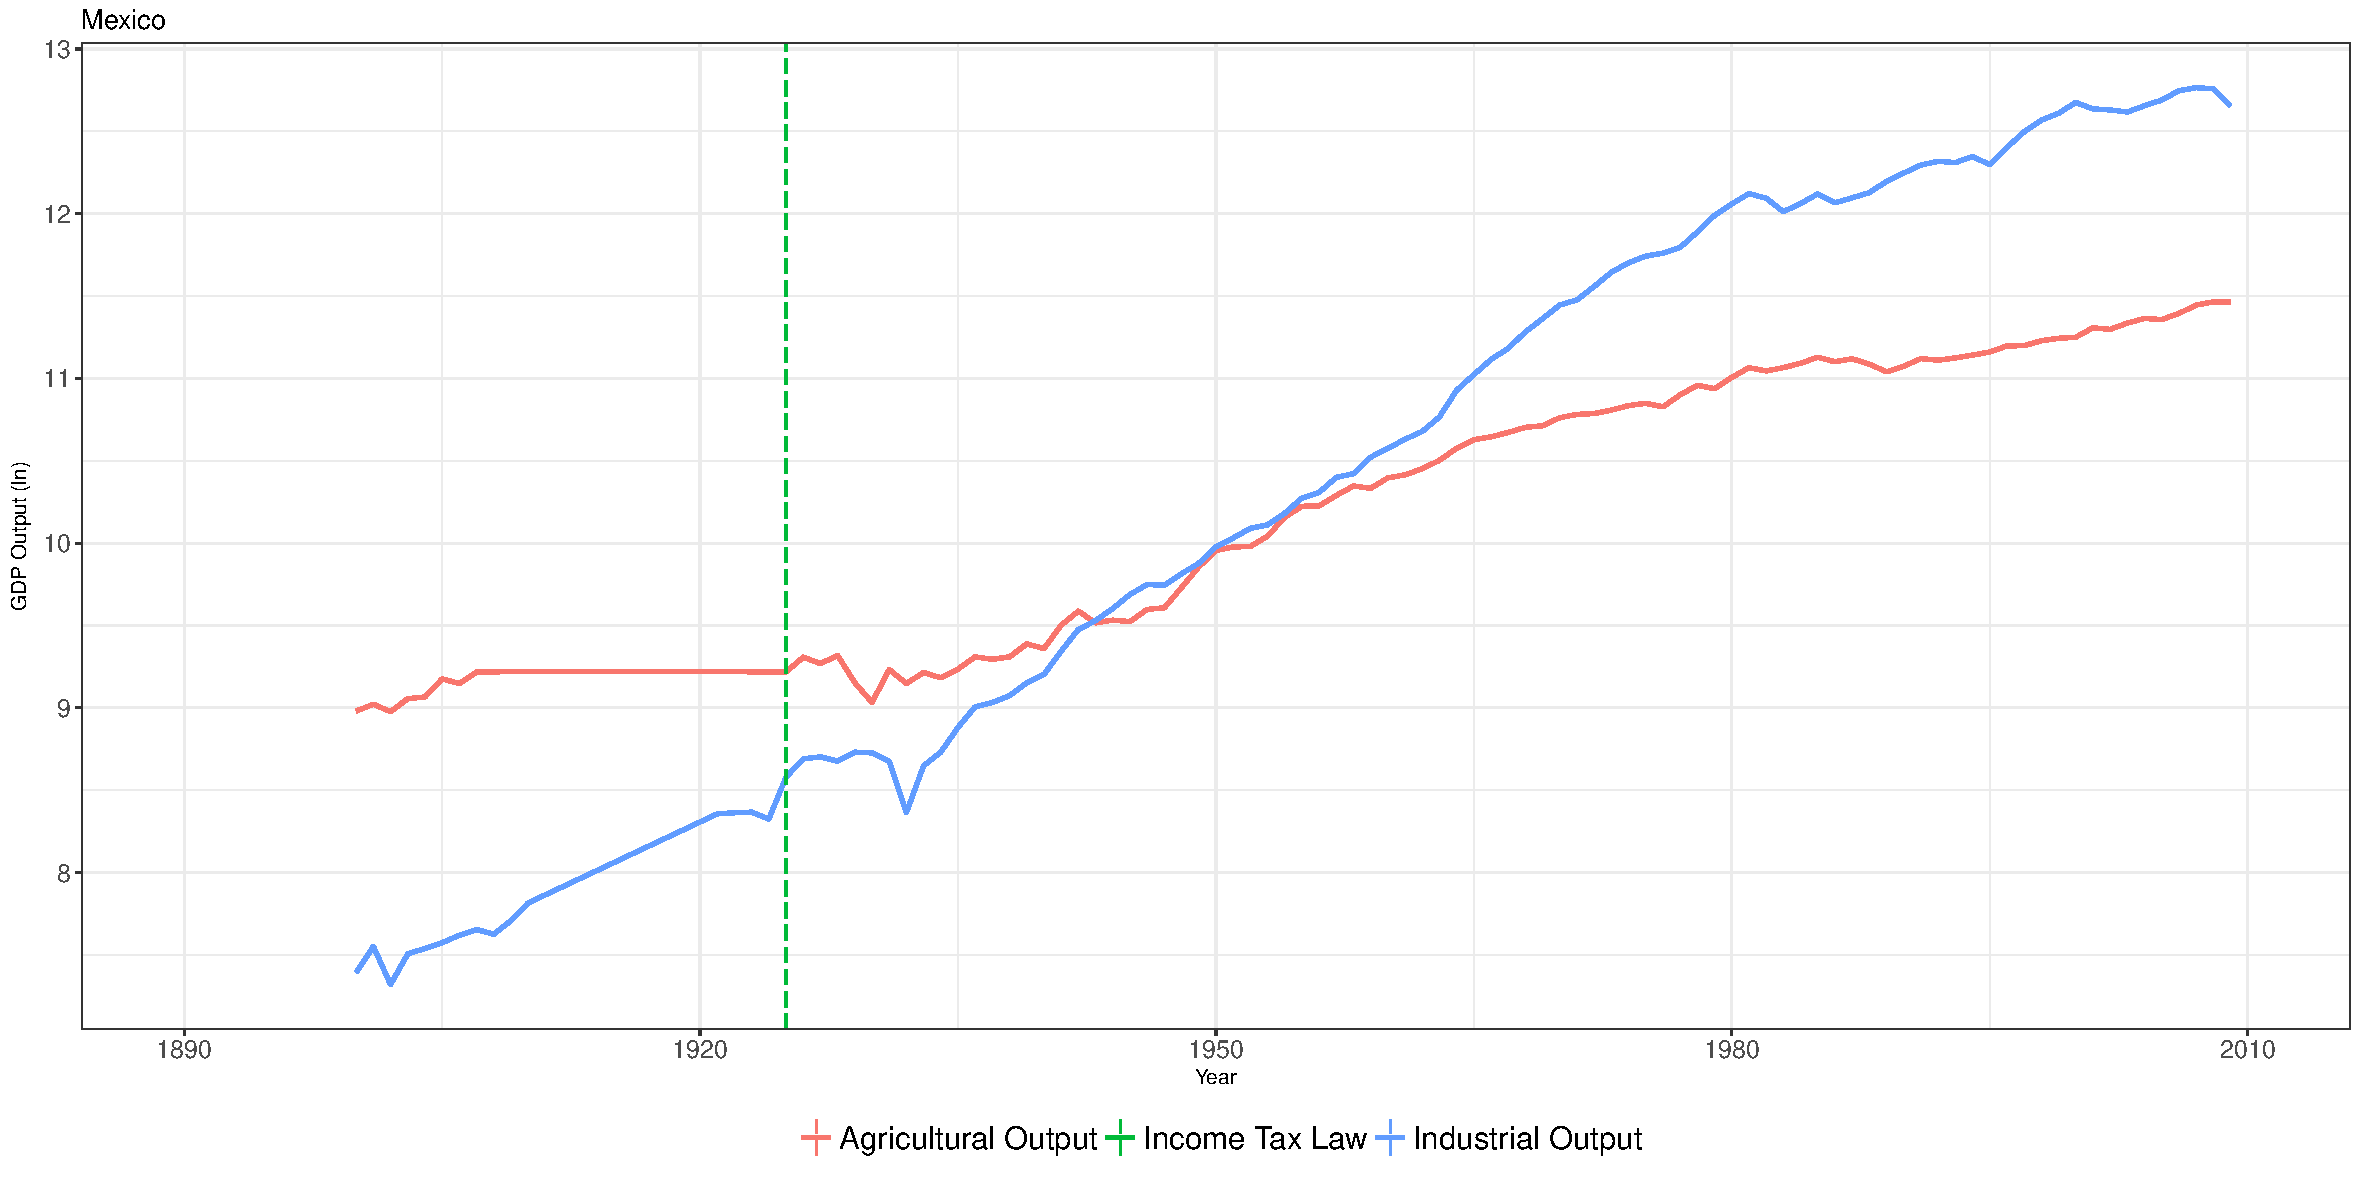
\includegraphics[scale=0.3]{/Users/hectorbahamonde/RU/Dissertation/Papers/IncomeTaxAdoption/Mexico_Income_Tax.pdf}
     \end{figure}
\end{frame}


\miniframesoff
\begin{frame}[plain]\frametitle{Argentina: 1933}
     \begin{figure}[H]
  %   \vspace{4mm}
  %   \hspace{-7.5mm}
  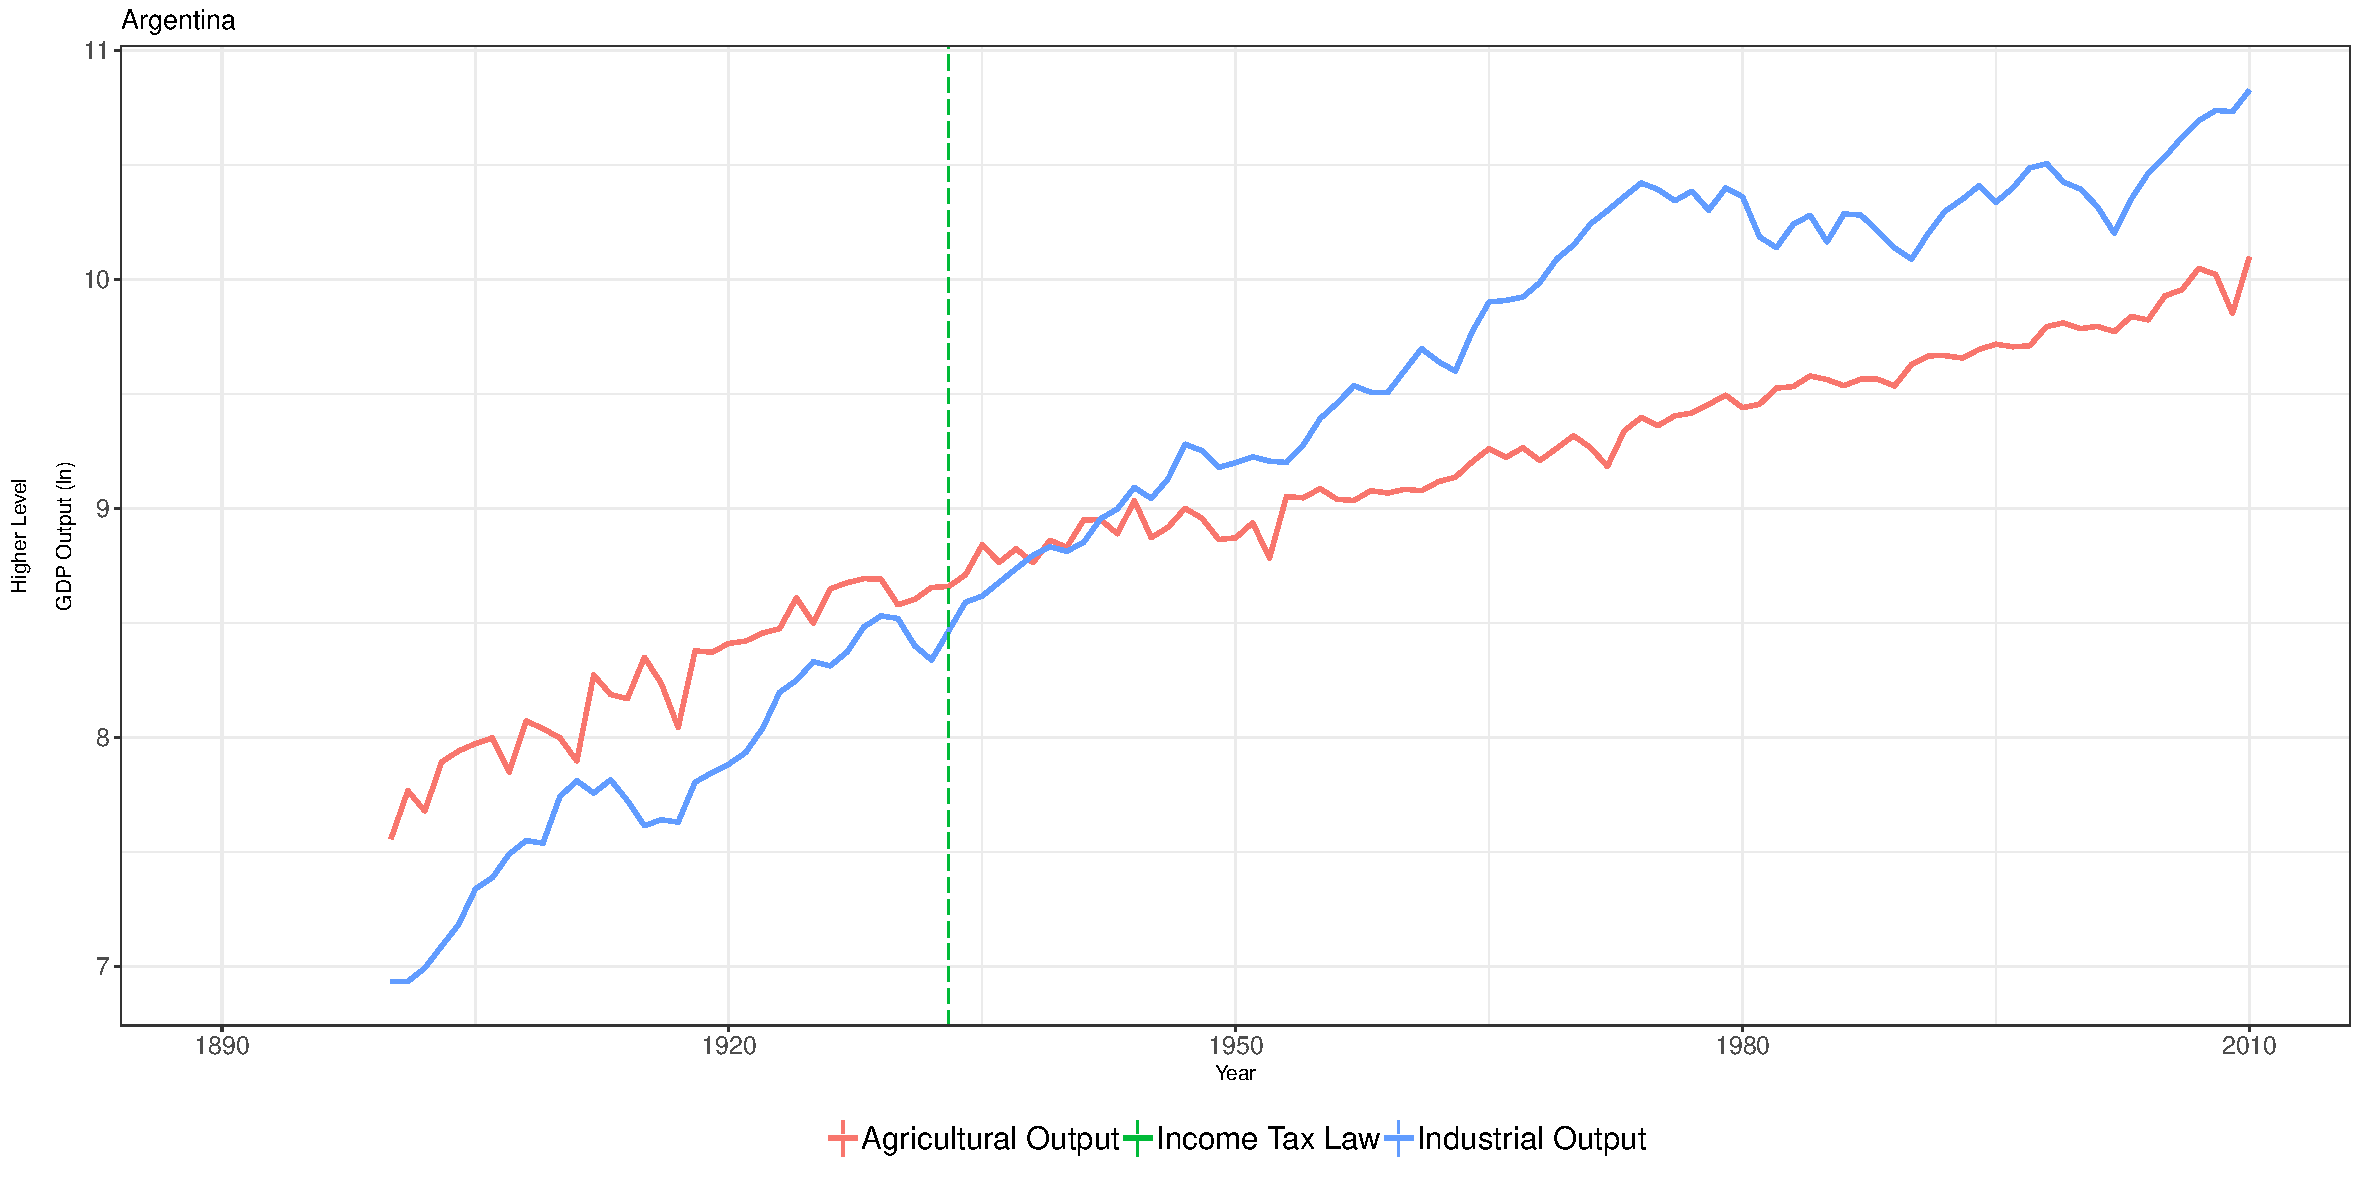
\includegraphics[scale=0.3]{/Users/hectorbahamonde/RU/Dissertation/Papers/IncomeTaxAdoption/Argentina_Income_Tax.pdf}
     \end{figure}
\end{frame}


\miniframesoff
\begin{frame}[plain]\frametitle{Guatemala: 1963}
     \begin{figure}[H]
  %   \vspace{4mm}
  %   \hspace{-7.5mm}
  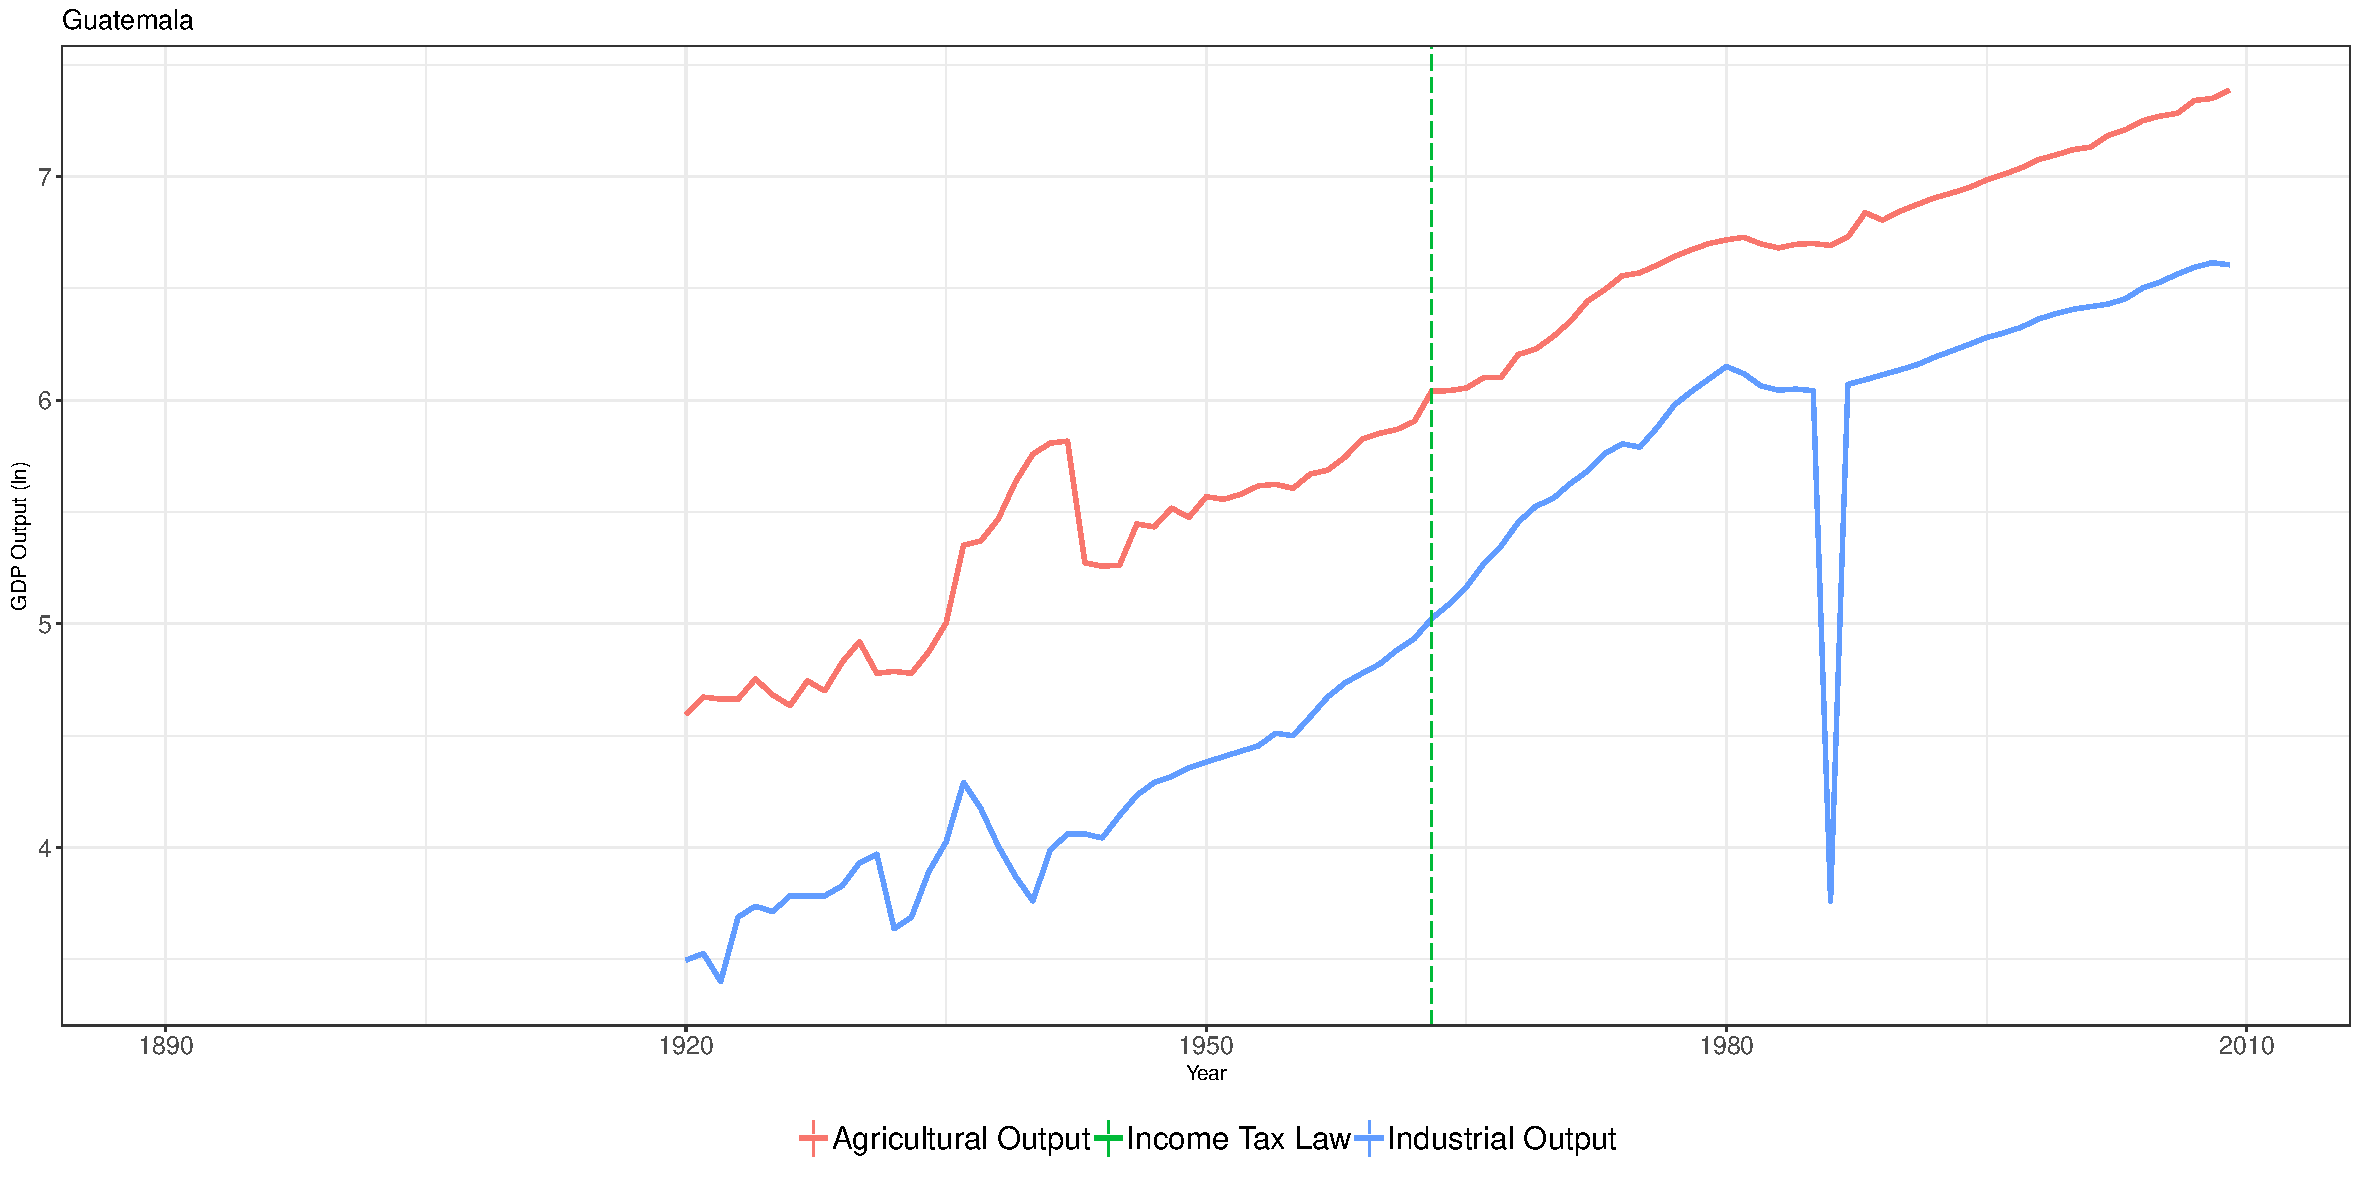
\includegraphics[scale=0.3]{/Users/hectorbahamonde/RU/Dissertation/Papers/IncomeTaxAdoption/Guatemala_Income_Tax.pdf}
     \end{figure}
\end{frame}


\miniframesoff
\begin{frame}[plain]\frametitle{Nicaragua: 1974}
     \begin{figure}[H]
  %   \vspace{4mm}
  %   \hspace{-7.5mm}
  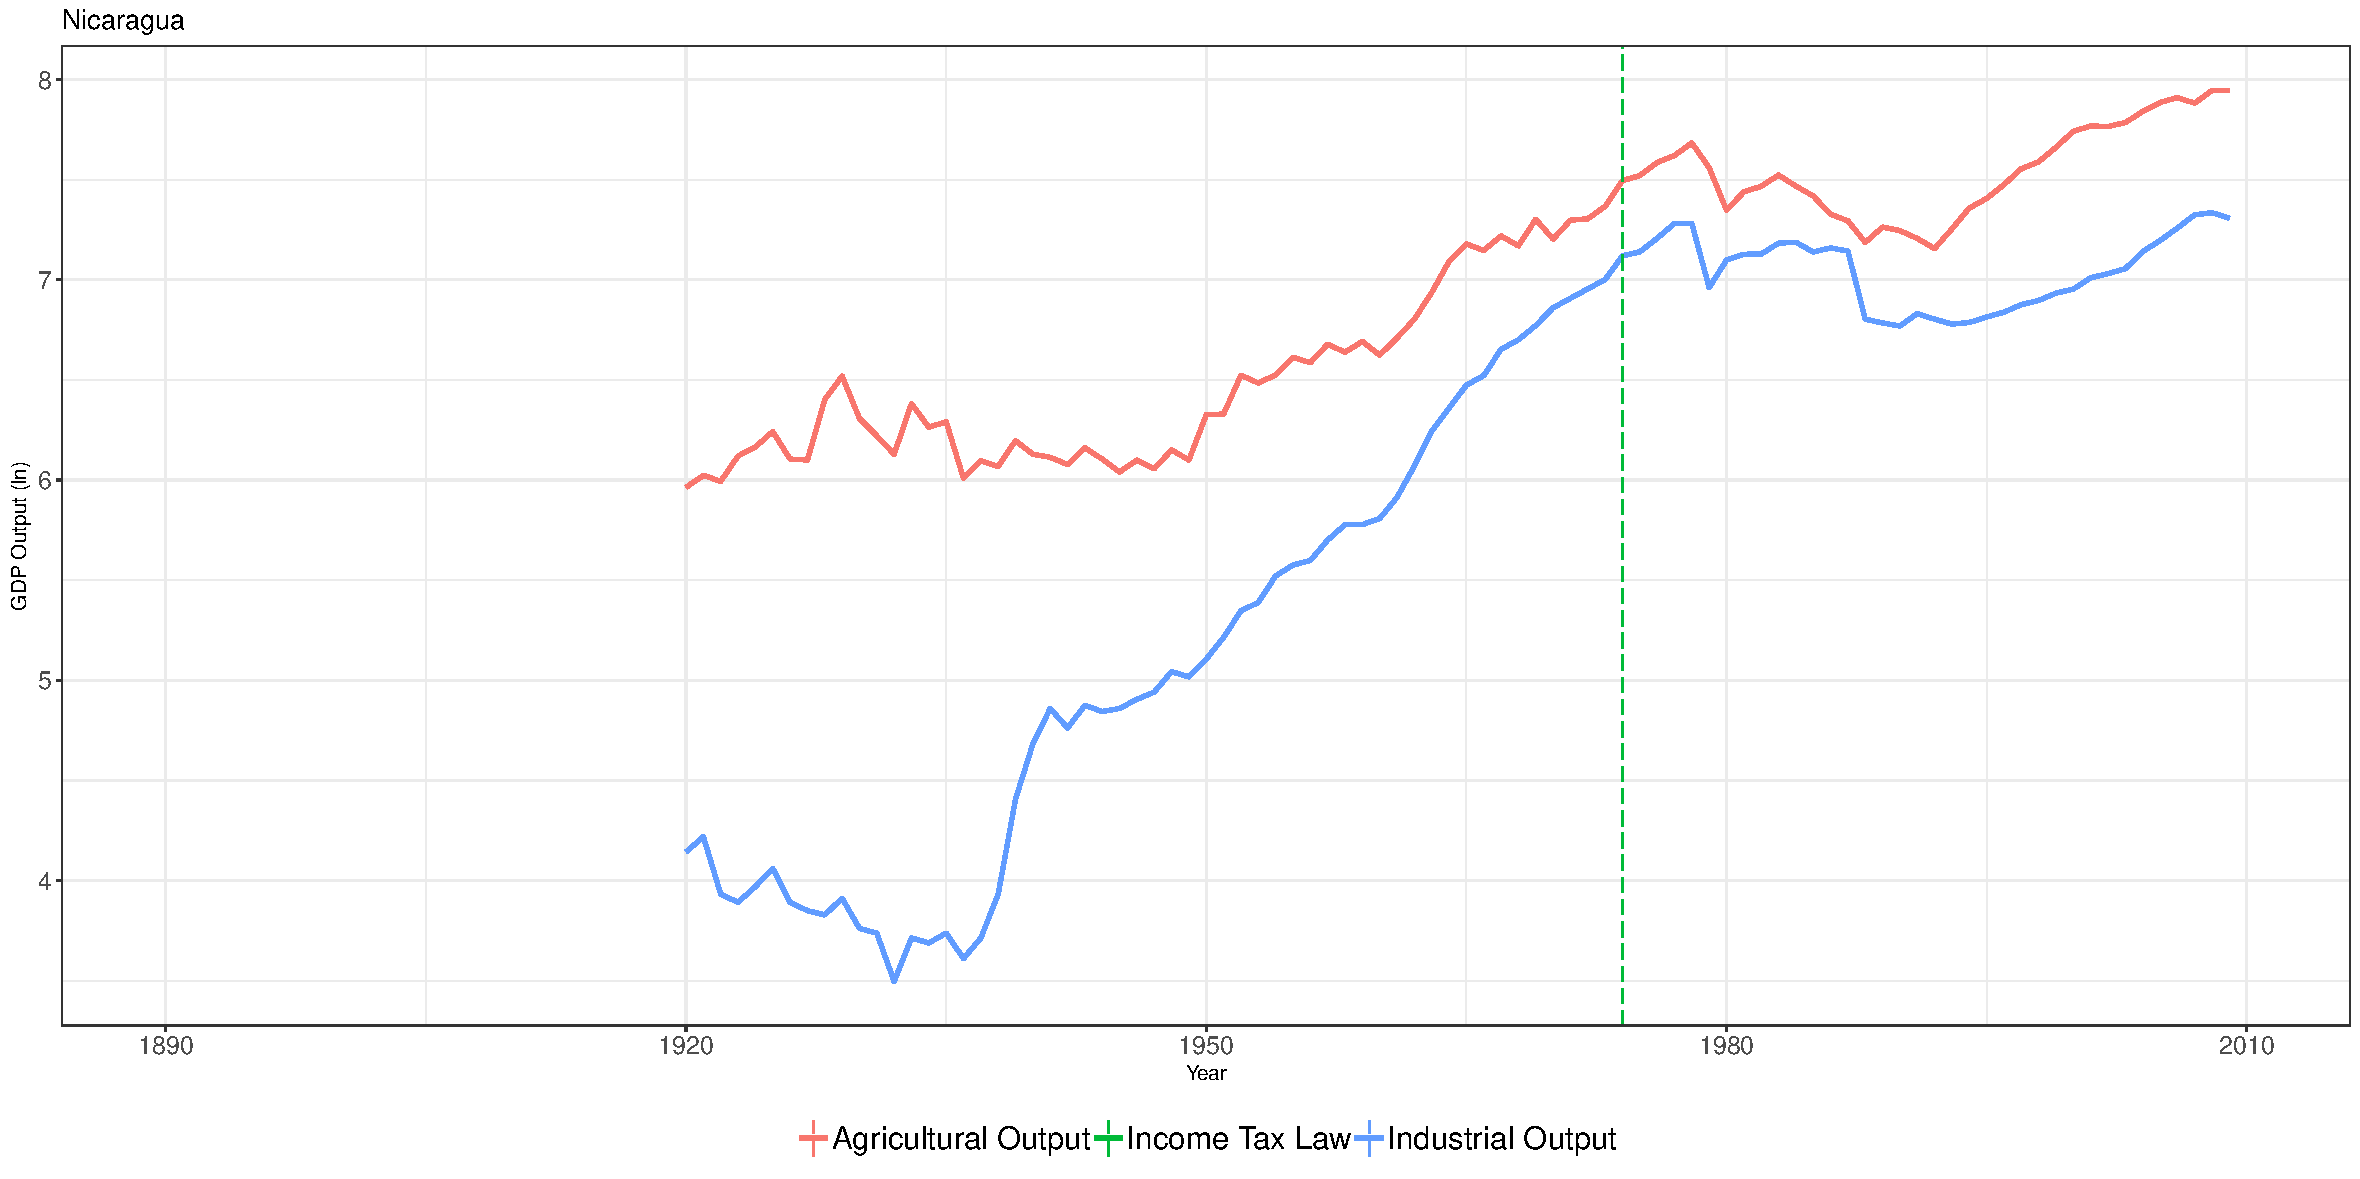
\includegraphics[scale=0.3]{/Users/hectorbahamonde/RU/Dissertation/Papers/IncomeTaxAdoption/Nicaragua_Income_Tax.pdf}
     \end{figure}
\end{frame}


\miniframesoff
\begin{frame}[plain]\frametitle{Venezuela: 1943}
     \begin{figure}[H]
  %   \vspace{4mm}
  %   \hspace{-7.5mm}
  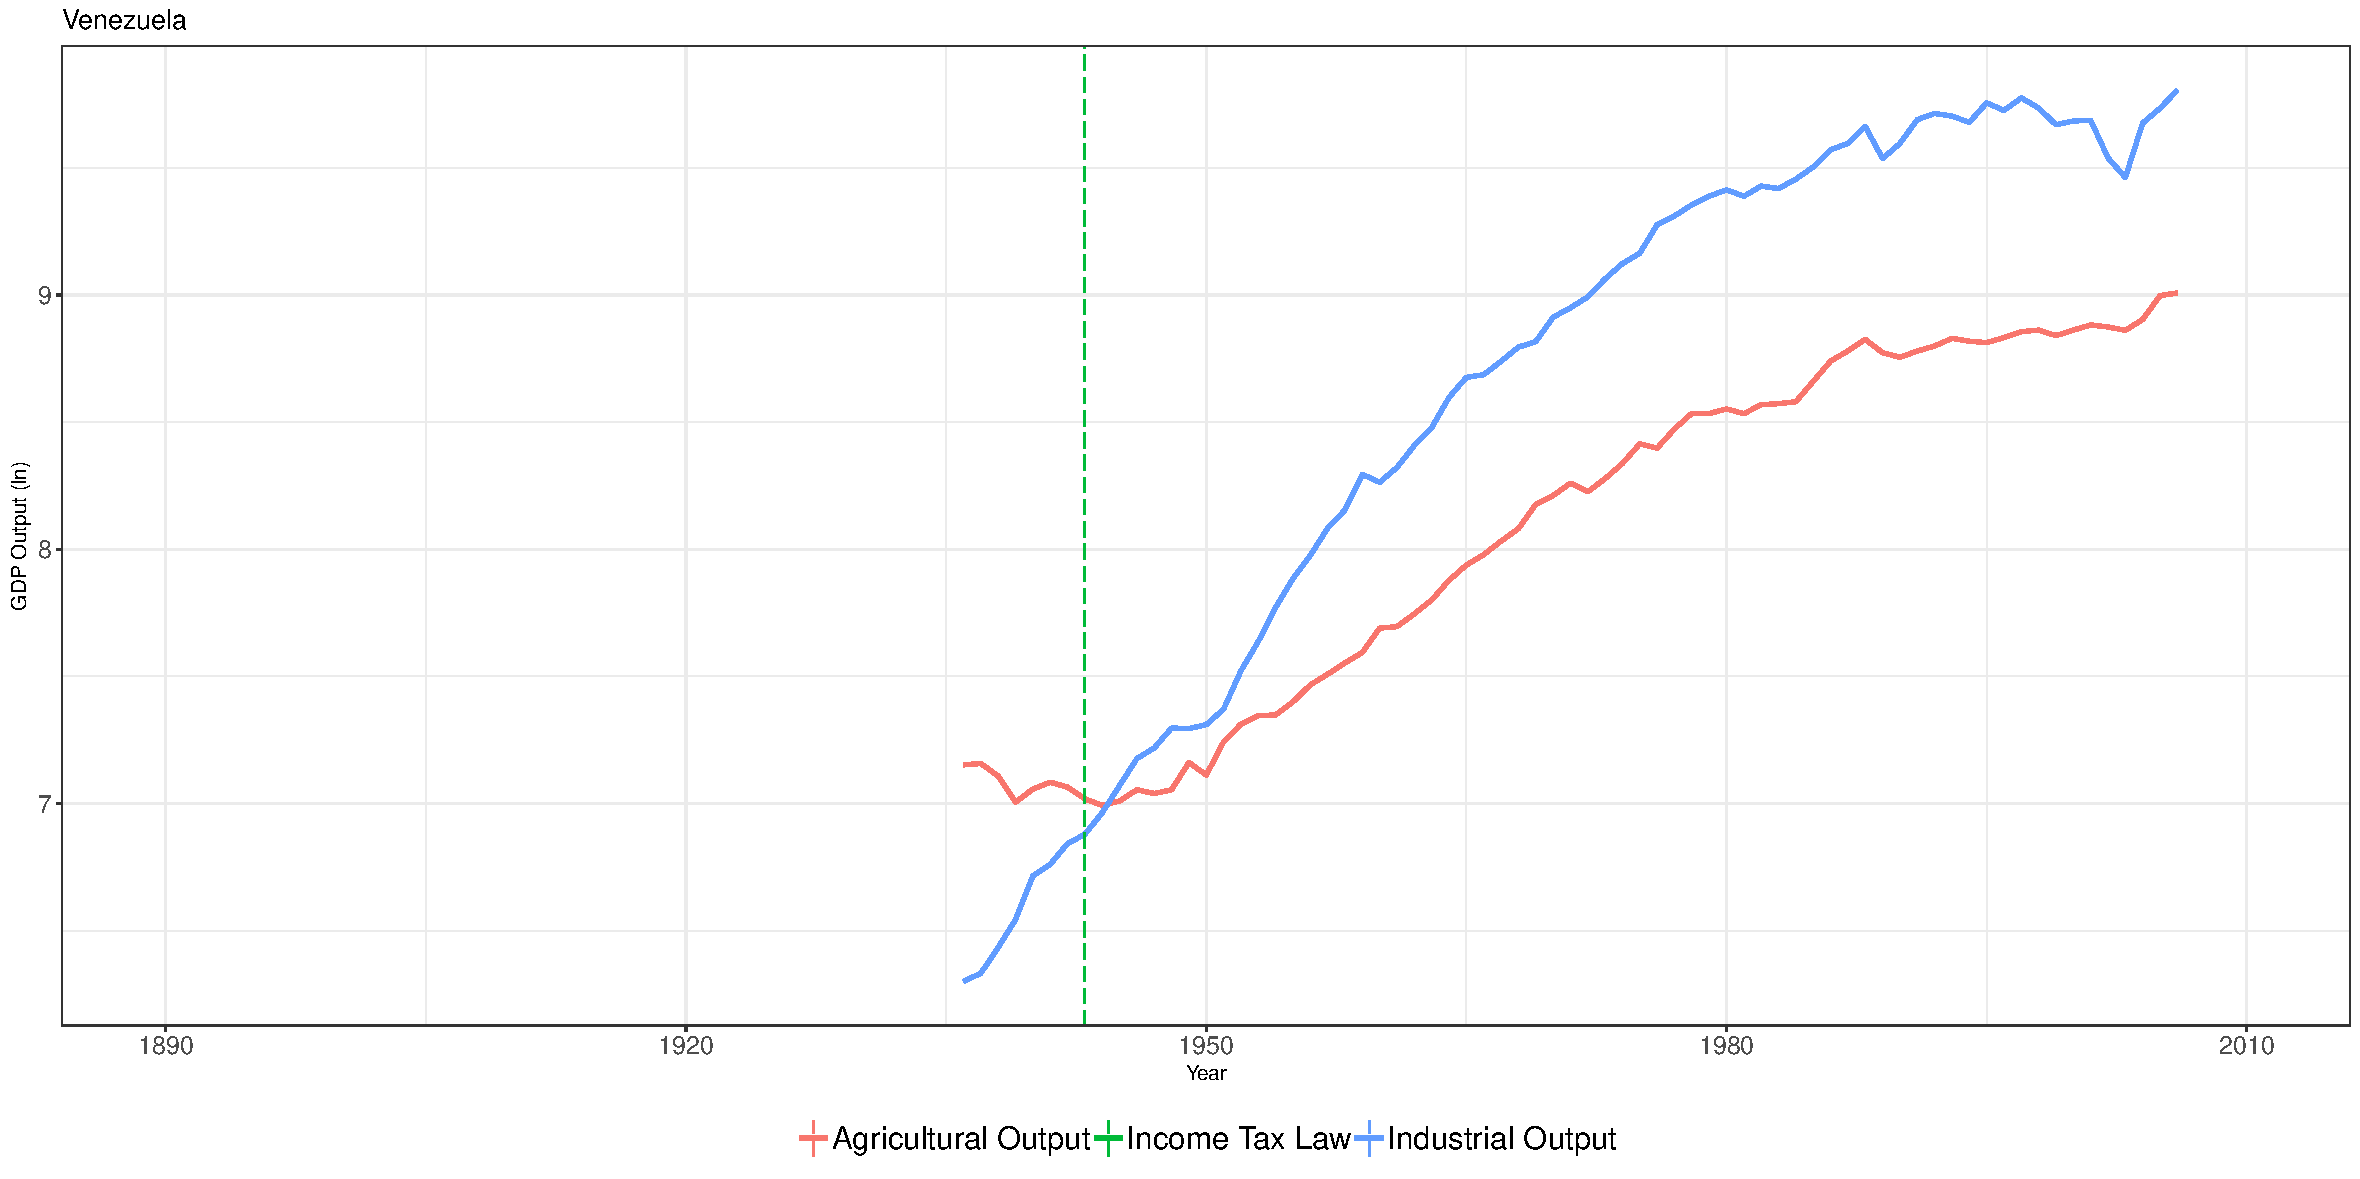
\includegraphics[scale=0.3]{/Users/hectorbahamonde/RU/Dissertation/Papers/IncomeTaxAdoption/Venezuela_Income_Tax.pdf}
     \end{figure}
\end{frame}



\miniframesoff
\begin{frame}[plain]\frametitle{Ecuador: 1945}
     \begin{figure}[H]
  %   \vspace{4mm}
  %   \hspace{-7.5mm}
  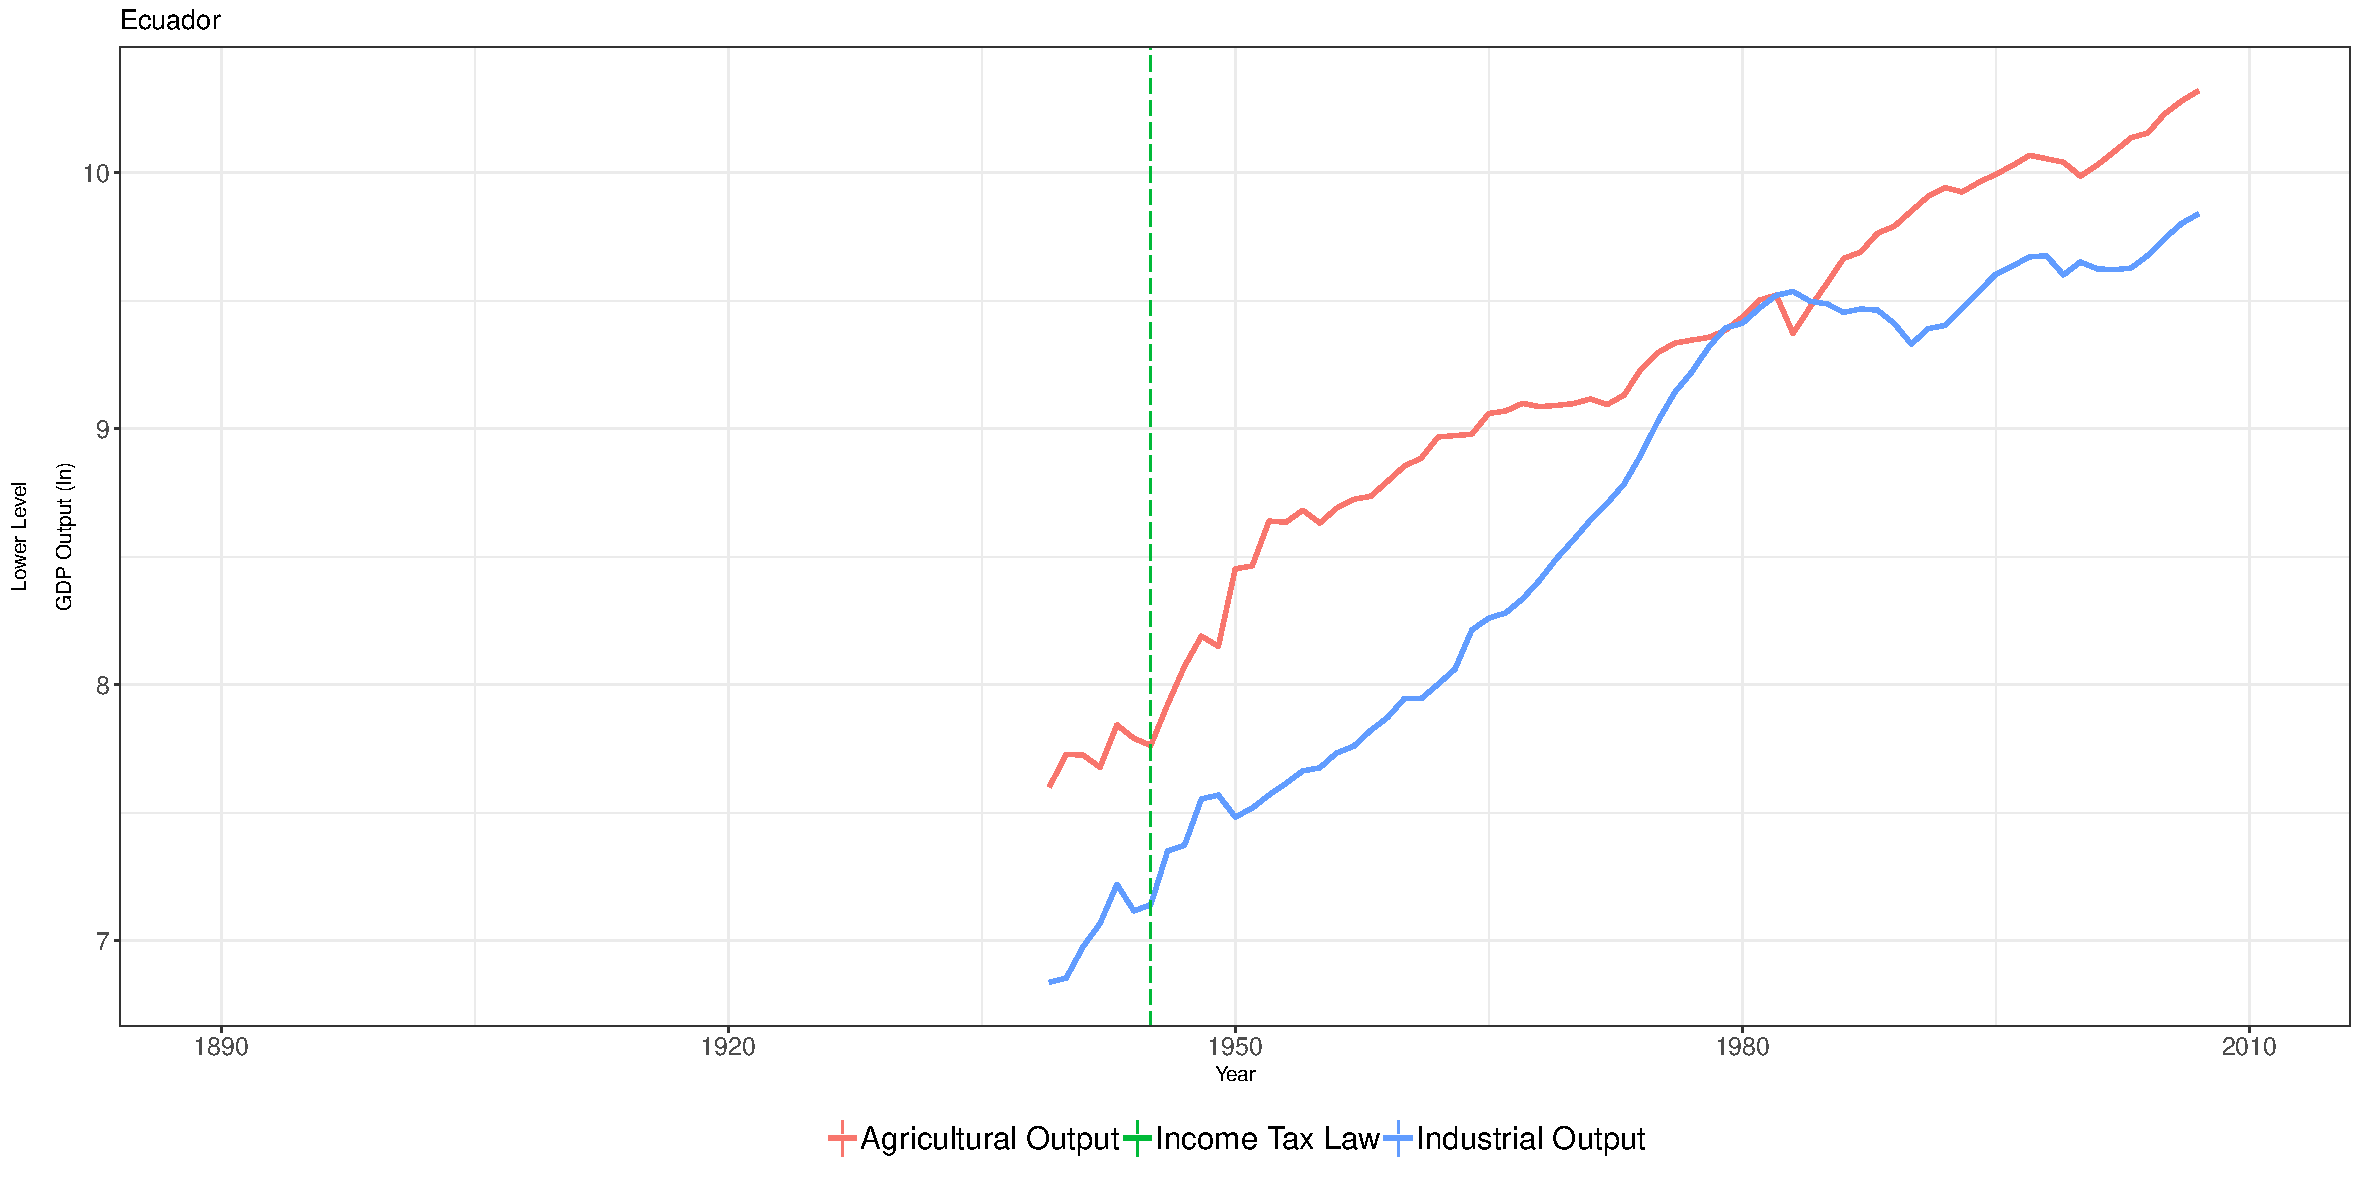
\includegraphics[scale=0.3]{/Users/hectorbahamonde/RU/Dissertation/Papers/IncomeTaxAdoption/Ecuador_Income_Tax.pdf}
     \end{figure}
\end{frame}



\miniframesoff
\begin{frame}[plain]\frametitle{Colombia: 1935}
     \begin{figure}[H]
  %   \vspace{4mm}
  %   \hspace{-7.5mm}
  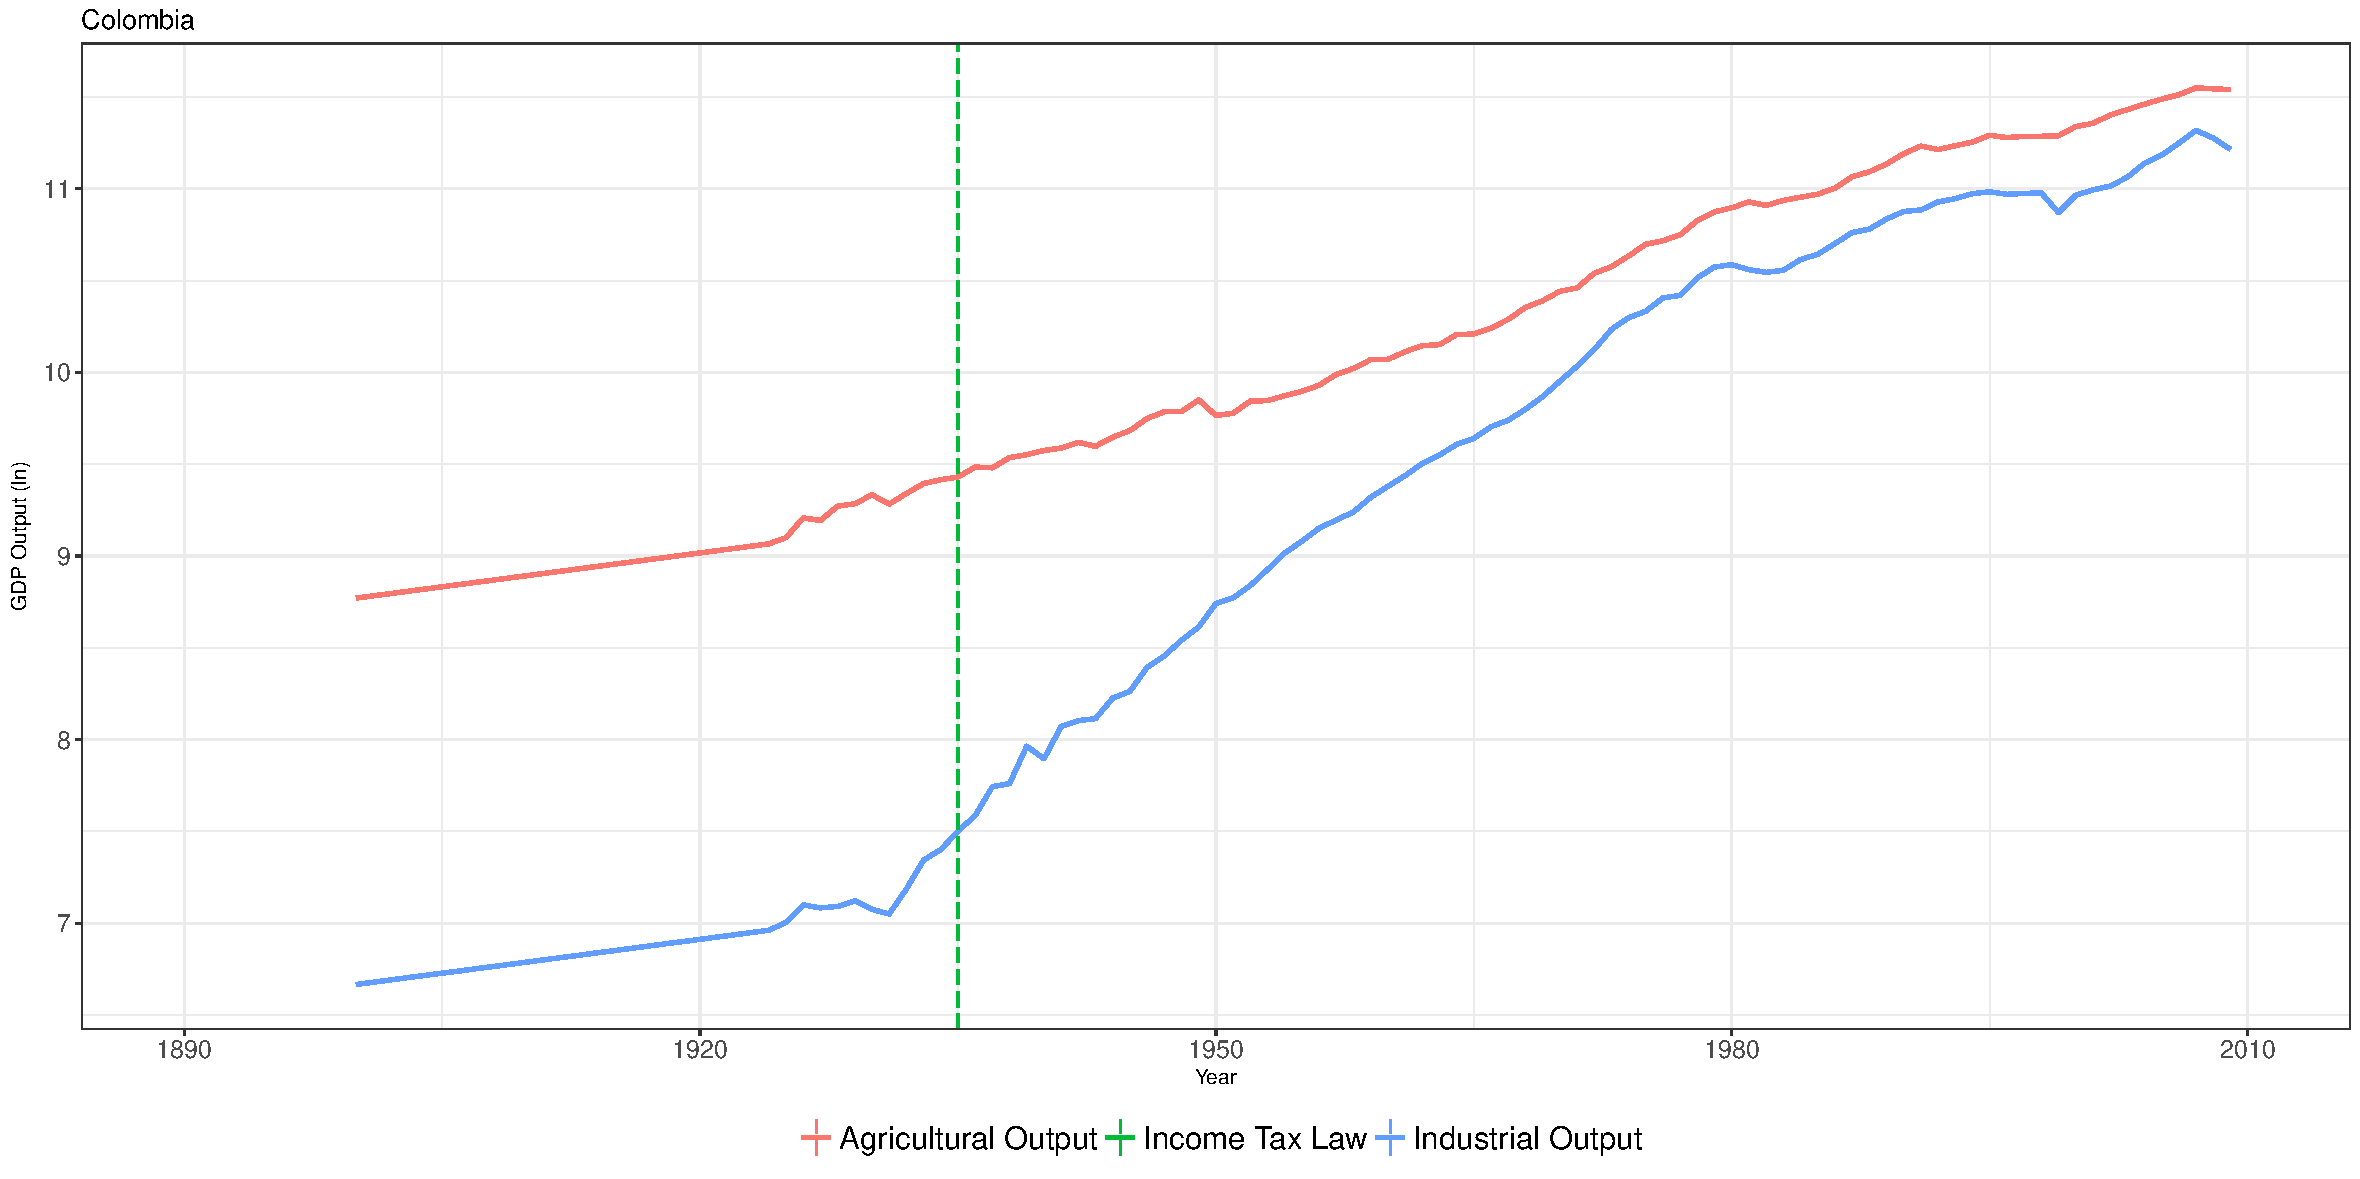
\includegraphics[scale=0.3]{/Users/hectorbahamonde/RU/Dissertation/Papers/IncomeTaxAdoption/Colombia_Income_Tax.pdf}
     \end{figure}
\end{frame}


\miniframesoff
\begin{frame}[plain]\frametitle{Peru: 1934}
     \begin{figure}[H]
  %   \vspace{4mm}
  %   \hspace{-7.5mm}
  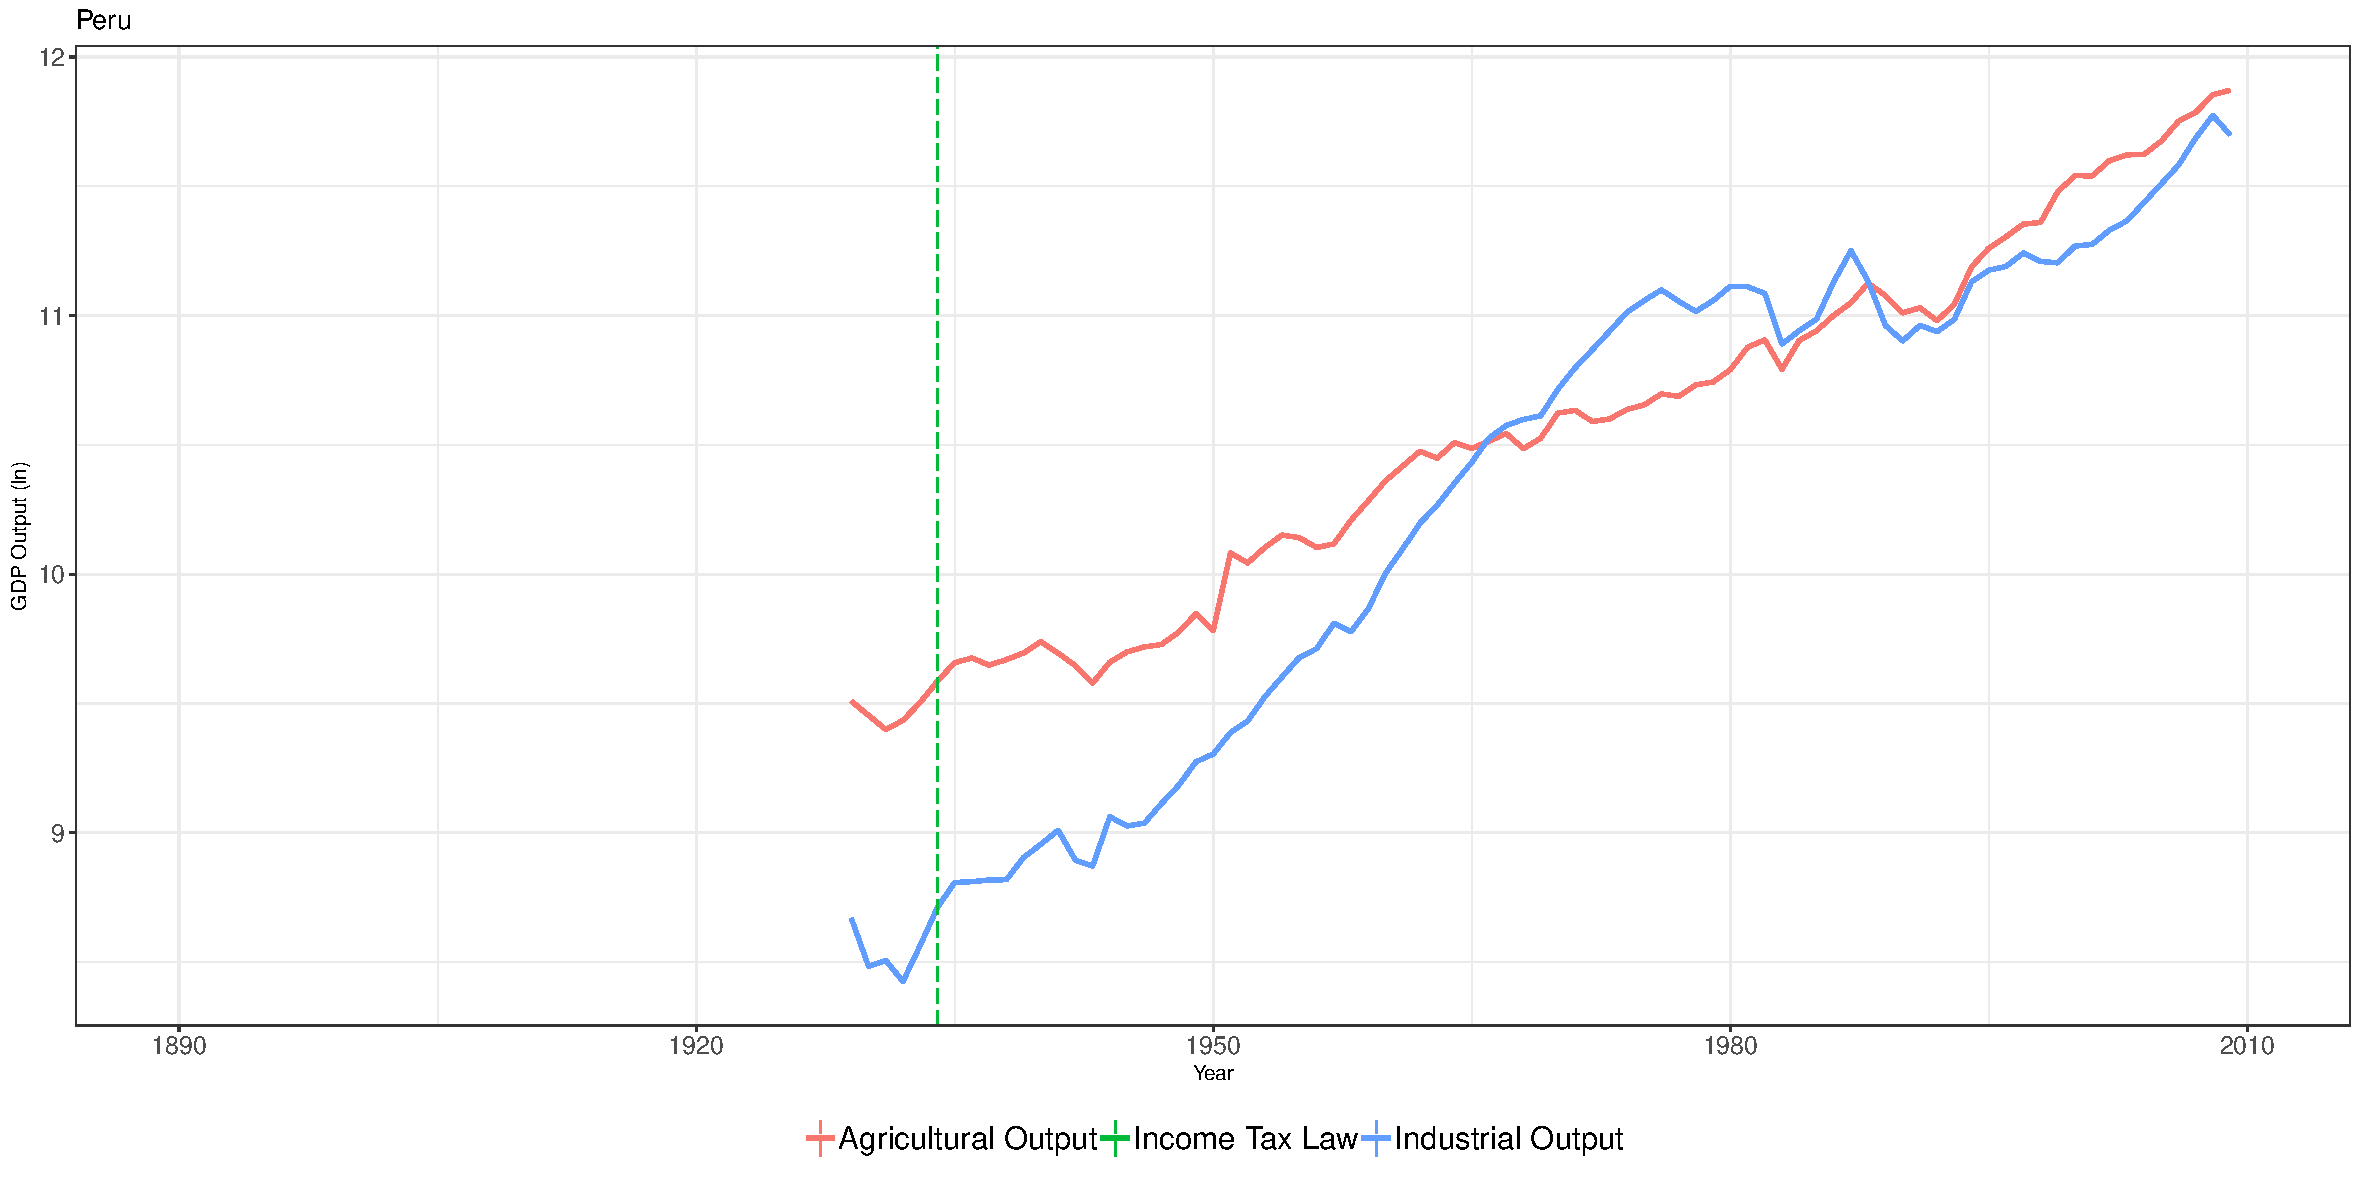
\includegraphics[scale=0.3]{/Users/hectorbahamonde/RU/Dissertation/Papers/IncomeTaxAdoption/Peru_Income_Tax.pdf}
     \end{figure}
\end{frame}


\miniframesoff
\begin{frame}[plain]\frametitle{Chile: 1924}
     \begin{figure}[H]
  %   \vspace{4mm}
  %   \hspace{-7.5mm}
  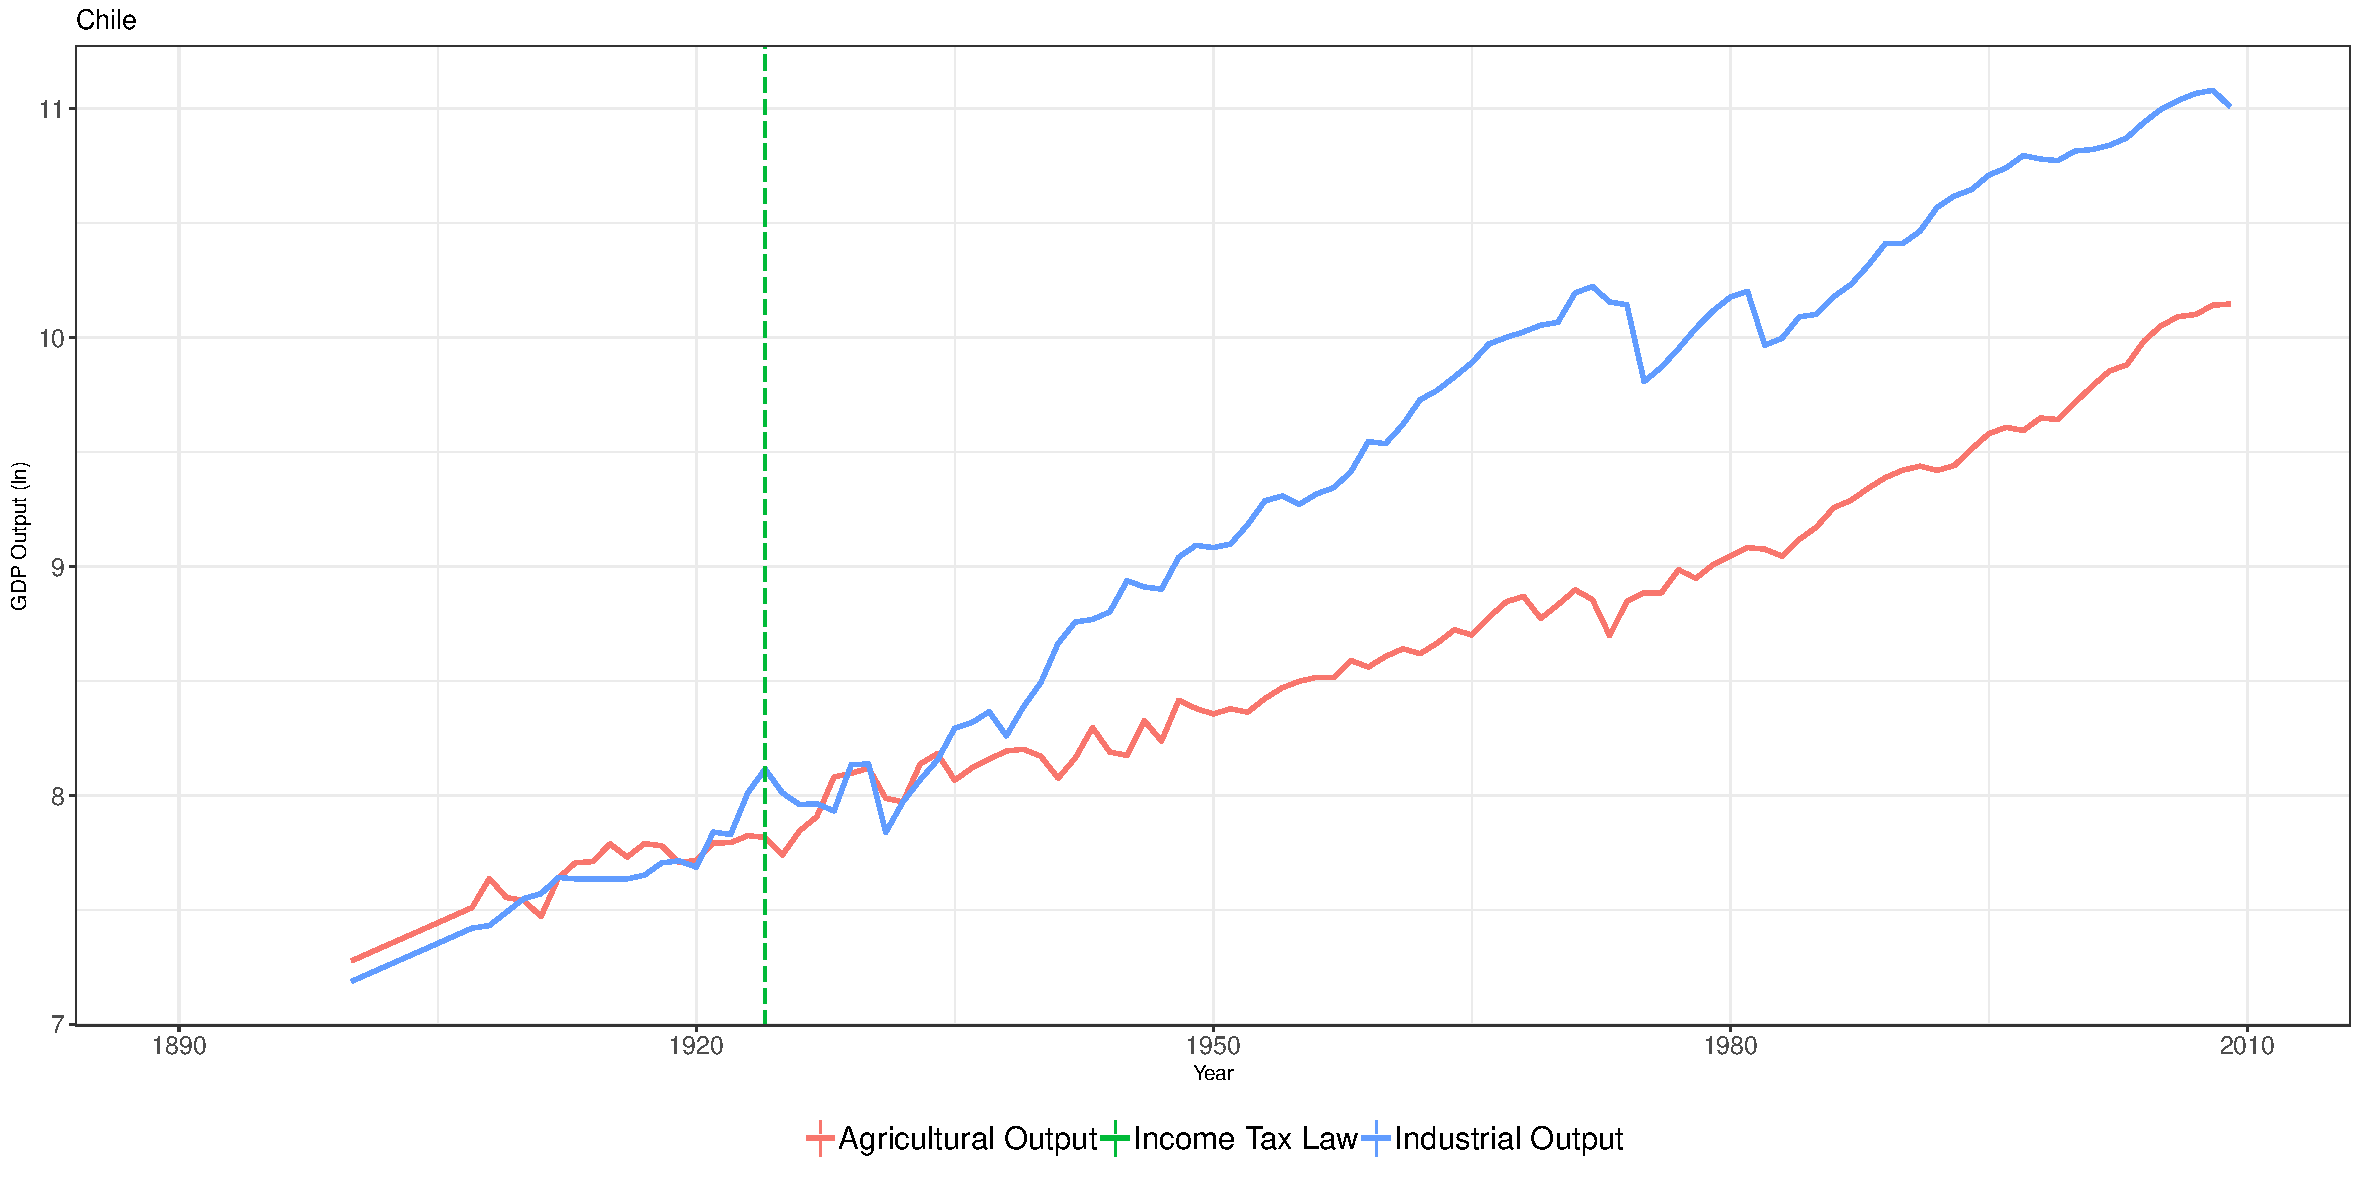
\includegraphics[scale=0.3]{/Users/hectorbahamonde/RU/Dissertation/Papers/IncomeTaxAdoption/Chile_Income_Tax.pdf}
     \end{figure}
\end{frame}


\subsection{Technical Details: Count Model}


\miniframeson
\begin{frame}\frametitle{State Capacities Overtime in Chile}

{\bf {\footnotesize Bayesian Poisson model with year fixed-effects. \hyperlink{jags_code}{\beamerbutton{Jags Code}}}}

\begin{equation*}
  \begin{array}{ll}
\text{Deaths} & \;\sim\; \text{Poisson}(\lambda_{i}) \hspace{4.1cm}\hyperlink{death_count_plot}{\beamerbutton{Distribution of Deaths}}
\vspace{5mm}
\\
log(\lambda_{i})  &= 
\;\mu + 
\beta_{1}\text{Income Tax}_{i,t} + 
\beta_{2}\text{Magnitude}^2_{i,t} +
\beta_{3}\text{Latitude}_{i,t} + \\
&\beta_{4}\text{Longitude}_{i,t} +
\beta_{5}\text{Population}_{i,t} +
\beta_{6}\text{Urban}_{i,t} + 
\beta_{7}\text{Year}_{t}
  \end{array}
\end{equation*}


{\small where,}

\footnotesize
\begin{equation*} 
\begin{split}
i_{1,...I} & \; \text{where} \; \text{I}=91\;\text{earthquakes}\\
t_{1,...T} & \; \text{where} \; \text{T}=59\;\text{years.}
\end{split}
\end{equation*}

\normalsize




\begin{itemize}
  \item[] {\tiny 4 chains, 200K iterations, burn-in of 5000}.
  \item[] \vspace{5mm}
  \hspace{-1cm} 
  \hyperlink{density_plot_tax}{\beamerbutton{Densities}} \hyperlink{trace_plot_tax}{\beamerbutton{Trace plots}} \hyperlink{model_fit}{\beamerbutton{Model fit}} \hyperlink{table_tax}{\beamerbutton{Reg Table}}  \href{https://github.com/hbahamonde/Earthquake_Paper/raw/master/Bahamonde_Earthquake_Paper_Diagnostic_Plots_Income_Tax_Model.pdf}{\beamerbutton{Download detailed diagnostics plots}}
\end{itemize}
\end{frame}






\miniframesoff
\begin{frame}\frametitle{State Capacities Overtime in Chile}

{\bf {\footnotesize Bayesian Poisson model with year fixed-effects. \hyperlink{jags_code}{\beamerbutton{Jags Code}}}}

\begin{equation*}
  \begin{array}{ll}
\text{Deaths} & \;\sim\; \text{Poisson}(\lambda_{i}) \hspace{4.1cm}\hyperlink{death_count_plot}{\beamerbutton{Distribution of Deaths}}
\vspace{5mm}
\\
log(\lambda_{i})  &= 
\;\mu + 
\beta_{1}\text{{\color{red}Income Tax}}_{i,t} + 
\beta_{2}\text{Magnitude}^2_{i,t} +
\beta_{3}\text{Latitude}_{i,t} + \\
&\beta_{4}\text{Longitude}_{i,t} +
\beta_{5}\text{Population}_{i,t} +
\beta_{6}\text{Urban}_{i,t} + 
\beta_{7}\text{Year}_{t}
  \end{array}
\end{equation*}


{\small where,}

\footnotesize
\begin{equation*} 
\begin{split}
i_{1,...I} & \; \text{where} \; \text{I}=91\;\text{earthquakes}\\
t_{1,...T} & \; \text{where} \; \text{T}=59\;\text{years.}
\end{split}
\end{equation*}

\normalsize




\begin{itemize}
	\item[] {\tiny 4 chains, 200K iterations, burn-in of 5000}.
	\item[] \vspace{5mm}
	\hspace{-1cm} 
	\hyperlink{density_plot_tax}{\beamerbutton{Densities}} \hyperlink{trace_plot_tax}{\beamerbutton{Trace plots}} \hyperlink{model_fit}{\beamerbutton{Model fit}} \hyperlink{table_tax}{\beamerbutton{Reg Table}}  \href{https://github.com/hbahamonde/Earthquake_Paper/raw/master/Bahamonde_Earthquake_Paper_Diagnostic_Plots_Income_Tax_Model.pdf}{\beamerbutton{Download detailed diagnostics plots}}
\end{itemize}
\end{frame}


\miniframesoff
\begin{frame}[plain]\frametitle{{\large Geographic Distribution of EQs }}
 %\hspace{-1.16cm}
  \centering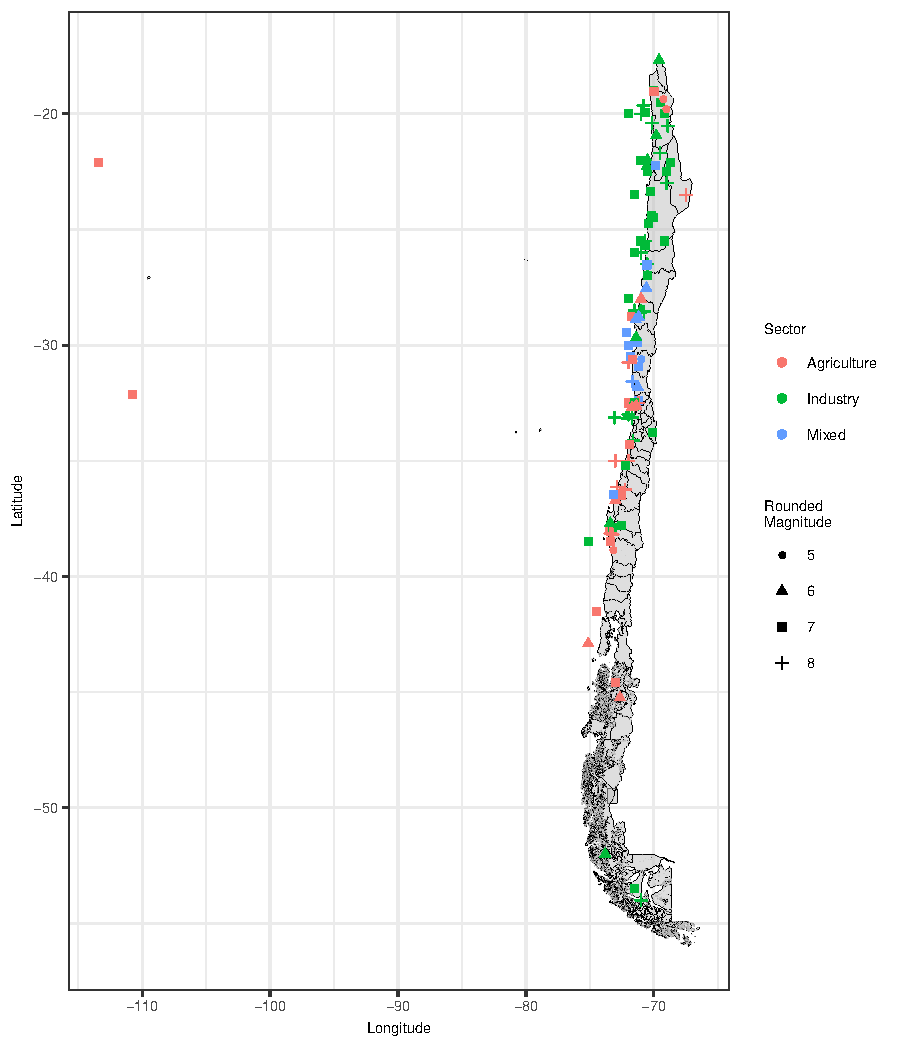
\includegraphics[scale=0.4]{/Users/hectorbahamonde/RU/Dissertation/Papers/Earthquake_Paper/figure/earthquake:map:plot:chile-1.pdf}
\end{frame}


\miniframesoff
\begin{frame}[plain]\frametitle{{\large Temporal Distribution of EQs}}
 %\hspace{-1.16cm}
  \centering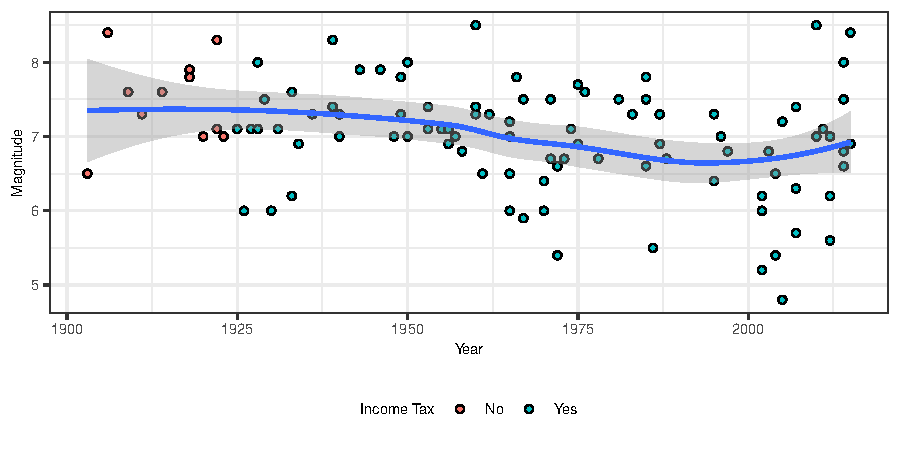
\includegraphics[scale=0.75]{/Users/hectorbahamonde/RU/Dissertation/Papers/Earthquake_Paper/figure/earthquake:ts:plot:chile:plot-1.pdf}
\end{frame}


\miniframesoff
\begin{frame}[plain]
\centering\huge Results
\end{frame}


\miniframeson
\subsection{Results: Early and Late Implementers}

\begin{frame}[plain]\frametitle{{\large Sectoral Contestation, and the Timing of the Income Tax Law {\scriptsize (9 Lat Am Count)}}}
 %\hspace{-1.16cm}
  \centering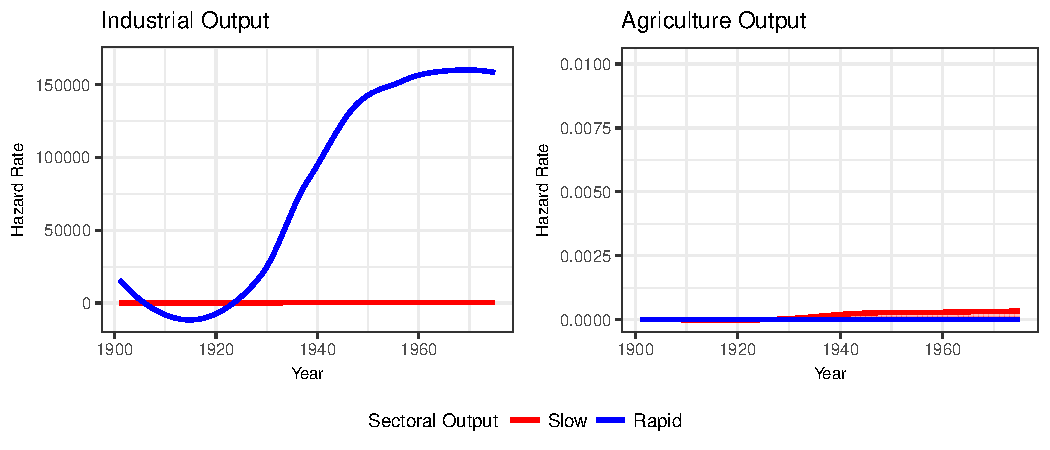
\includegraphics[scale=0.75]{/Users/hectorbahamonde/RU/Dissertation/Papers/Earthquake_Paper/figure/simulation:plots-1.pdf}

    \hyperlink{duration_models}{\beamerbutton{reg table}}

\end{frame}


\miniframeson
\subsection{Results: State Capacities Overtime}


\begin{frame}[plain]\frametitle{{\large Income Taxation Increases State Development Overtime {\scriptsize (Chile)}}}
 %\hspace{-1.16cm}
  \centering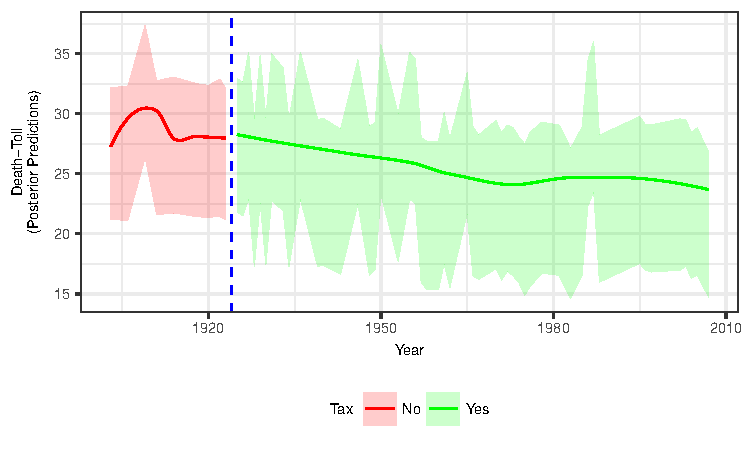
\includegraphics[scale=0.75]{/Users/hectorbahamonde/RU/Dissertation/Papers/Earthquake_Paper/figure/income:tax:model:plot:run-1.pdf}
      \hyperlink{table_tax}{\beamerbutton{reg table}}

\end{frame}



\section{Summary}
\miniframeson

\subsection{Summary}


% Summary frame
\miniframesoff
\begin{frame}\frametitle{Summary}
	\begin{enumerate}
		 \item The {\bf emergence of a strong industrial sector}, accelerated the implementation of the \emph{income tax} in nine countries in Latin America.

		 \item {\bf Income taxation} increased \emph{state capacities} overtime in Chile.

	\end{enumerate} 

\pause

Why care?
  
  \begin{enumerate}
     \item {\bf A novel earthquake dataset} was used to measure state capacities overtime. \pause Under reasonable assumptions, the capacity of a state to enforce building codes, is a reflection of its overall state capacity. \pause

     \item \emph{Unlike} other theories, my paper stressed the {\bf domestic factors} at play {\scriptsize(\emph{sectoral contestion})}, relaxing the conflict---\emph{Tillian}---hypothesis.
  \end{enumerate} 


\end{frame}



\begin{frame}[plain,c, label=thank_you]



\miniframesoff
\begin{center}
\Huge{Thank you}\\
\vspace{1cm} \texttt{www.Hector{\color{black!30!green}{\bf Bahamonde}}.com}
\end{center}
\vspace{1cm}
% \hspace{5cm}
\centering\scalebox{0.7}{\hyperlink{toc}{\beamerbutton{TOC}}}
%\vspace{2cm}\hspace{5cm}
\centering\scalebox{0.7}{\hyperlink{cover}{\beamerbutton{Cover}}}
\end{frame}




%%%%%%%%%%%%%%%%%%%%%%%%%%%%%%%%%%%%%%%%%%%%%%%%%%%%%%%%%%%%%%%%%%%%%%%%%%
%%%%%%%%%%%%%%%%%%%%%%%%%%%%%%%%%%%%%%%%%%%%%%%%%%%%%%%%%%%%%%%%%%%%%%%%%%
%%%%%%%%%%%%%%%%%%%%%%%%%%%%%%%%%%%%%%%%%%%%%%%%%%%%%%%%%%%%%%%%%%%%%%%%%%
%%%%%%%%%%%%%%%%%%%%%%%%%%%%%%%%%%%%%%%%%%%%%%%%%%%%%%%%%%%%%%%%%%%%%%%%%%



\section{Appendix}
\miniframesoff




%%%%%%%%%%%%%%%%%%%%%%%%%%%%%%%%%%%%%%%%%%%%%%%%%%%%%%%%%%%%%%%%%%%%%%%%%%
\begin{frame}[label = toc]\frametitle{TOC}

\begin{columns}

\column{0.5\textwidth}


\Tiny{
	\begin{itemize}
		\item[] -\hyperlink{unit_root}{P2: Unit Root Tests}
		\item[] -\hyperlink{johansen_tests}{P2: Johansen Tests for Cointegration}
		\item[] -\hyperlink{lags_tests}{P2: Lags Tests}
		\item[] -\hyperlink{ts_plots}{P2: Sectoral Outputs}
		\item[] -\hyperlink{granger_test}{P2: Granger-causality Tests}
		\item[] -\hyperlink{density_plot_tax}{P3: Income Tax Model Density Plots}
		\item[] -\hyperlink{trace_plot_tax}{P3: Income Tax Model Trace Plots}
		\item[] -\hyperlink{model_fit}{P3: Sectoral and Income Tax Model Goodness of Fit Plot}
		\item[] -\hyperlink{table_sectoral}{P3: Sectoral Model Regression Table}
		\item[] -\hyperlink{table_tax}{P3: Income Tax Model Regression}
		\item[] -\hyperlink{jags_code}{P3: Jags code for sectoral model}
		\item[] -\hyperlink{death_count_plot}{P3: Distribution of Deaths} 
		\item[] -\hyperlink{credible_threats}{Credible Threats} 


	\end{itemize}
}	


\column{0.5\textwidth}
\Tiny{
	\begin{itemize}
		\item[] -\hyperlink{conflict}{From Conflict to Cooperation}
		\item[] -\hyperlink{1891_1924}{War was in 1891, but income tax was implemented in 1924}
		\item[] -\hyperlink{tax_sect_comp}{Why does taxation increase with sectoral competition?}
		\item[] -\hyperlink{origins_industry}{Everything depends on industrial expansion. Where does industry come from, then?}
		\item[] -\hyperlink{why_not_indirect_taxes}{Why not indirect taxation?}
		\item[] -\hyperlink{duration_models}{Duration Models}

	\end{itemize}
}

\end{columns}

\vspace{2cm}
% \hspace{5cm}
\centering\scalebox{0.7}{\hyperlink{thank_you}{\beamerbutton{Thank You}}}
%\vspace{2cm}\hspace{5cm}
\centering\scalebox{0.7}{\hyperlink{cover}{\beamerbutton{Cover}}}
\end{frame}
%%%%%%%%%%%%%%%%%%%%%%%%%%%%%%%%%%%%%%%%%%%%%%%%%%%%%%%%%%%%%%%%%%%%%%%%%%



%%%%%%%%%%%%%%%%%%%%%%%%%%%%%%%%%%%%%%%%%%%%%%%%%%%%%%%%%%%%%%%%%%%%%%%%%%%%%%%
\miniframesoff


\begin{frame}[label=duration_models,plain]%\frametitle{Duration Models}

\scalebox{0.62}{

% \centering
\hspace{10mm}
\begin{tabular}{c||c|c|c|c|c}
 & \multicolumn{1}{c|}{Cox (1 lag)} & \multicolumn{1}{c|}{Cox (1 lag, ln)} & \multicolumn{1}{c|}{Logit GEE} & \multicolumn{1}{c|}{Conditional Logit (FE)} & \multicolumn{1}{c}{Spatial Dependence} \\
\hline
\hline

Manufacture Output$_{t-1}$       & 4.923$^{**}$		&           		  &             	 &              	 &               	  \\
                                 & (1.851)    		&           		  &             	 &              	 &               	  \\
Agricultural Output$_{t-1}$      & -4.208$^{*}$ 	&           		  &             	 &              	 &               	  \\
                                 & (1.638)    		&           		  &             	 &              	 &               	  \\
Total Population                 & 0.000$^{**}$ 	&           		  &             	 &              	 &               	  \\
                                 & (0.000)    		&           		  &             	 &              	 &               	  \\
Manufacture Output$_{t-1}$ (ln)  &            		& 7.685$^{*}$ 		  &             	 &              	 &               	  \\
                                 &            		& (3.333)   		  &             	 &              	 &               	  \\
Agricultural Output$_{t-1}$ (ln) &            		& -6.971$^{*}$		  &             	 &              	 &               	  \\
                                 &            		& (3.227)   		  &             	 &              	 &               	  \\
Total Population (ln)            &            		& 5.059$^{*}$ 		  & 1.259       	 & 1.030$^{**}$   	 & 4.676$^{\cdot}$ 	  \\
                                 &            		& (2.228)   		  & (1.052)     	 & (0.391)      	 & (2.682)       	  \\
Manufacture Output (ln)          &            		&           		  & 1.924$^{***}$ 	 & 0.668$^{***}$  	 & 7.148         	  \\
                                 &            		&           		  & (0.514)     	 & (0.143)      	 & (4.815)       	  \\
Agricultural Output (ln)         &            		&           		  & -1.596$^{**}$ 	 & -0.941$^{***}$ 	 & -6.465        	  \\
                                 &            		&           		  & (0.603)     	 & (0.281)      	 & (4.636)       	  \\
\hline
AIC                              & 12.796     		& 10.894    		  &             	 & 4505.538     	 & 11.056        	  \\
R$^2$                            & 0.059      		& 0.068     		  &             	 & 0.341        	 & 0.065         	  \\
Max. R$^2$                       & 0.085      		& 0.088     		  &             	 & 0.997        	 & 0.085         	  \\
Num. events                      & 9          		& 9         		  &             	 & 610          	 & 9             	  \\
Num. obs.                        & 241        		& 232       		  & 842         	 & 842          	 & 241           	  \\
Missings                         & 0          		& 0         		  &             	 & 0            	 & 0             	  \\
PH test                          & 0.388      		& 0.877     		  &             	 &              	 & 0.667         	  \\
Num. clust.                      &            		&           		  & 9           	 &              	 &               	  \\
\hline
\multicolumn{6}{l}{\tiny{$^{***}p<0.001$, $^{**}p<0.01$, $^*p<0.05$, $^{\cdot}p<0.1$. Robust standard errors in all models}}
\end{tabular}
}
\end{frame}


% 5
\begin{frame}[plain]
\scalebox{0.62}{

%\centering
\hspace{10mm}
\begin{tabular}{c||c|c|c|c|c}
 & \multicolumn{1}{c|}{{\color{red}Cox (1 lag)}} & \multicolumn{1}{c|}{{\color{red}Cox (1 lag, ln)}} & \multicolumn{1}{c|}{{\color{red}Logit GEE}} & \multicolumn{1}{c|}{{\color{red}Conditional Logit (FE)}} & \multicolumn{1}{c}{{\color{red}Spatial Dependence}} \\
\hline
\hline

Manufacture Output$_{t-1}$       & 4.923$^{**}$		&           		  &             	 &              	 &               	  \\
                                 & (1.851)    		&           		  &             	 &              	 &               	  \\
Agricultural Output$_{t-1}$      & -4.208$^{*}$ 	&           		  &             	 &              	 &               	  \\
                                 & (1.638)    		&           		  &             	 &              	 &               	  \\
Total Population                 & 0.000$^{**}$ 	&           		  &             	 &              	 &               	  \\
                                 & (0.000)    		&           		  &             	 &              	 &               	  \\
Manufacture Output$_{t-1}$ (ln)  &            		& 7.685$^{*}$ 		  &             	 &              	 &               	  \\
                                 &            		& (3.333)   		  &             	 &              	 &               	  \\
Agricultural Output$_{t-1}$ (ln) &            		& -6.971$^{*}$		  &             	 &              	 &               	  \\
                                 &            		& (3.227)   		  &             	 &              	 &               	  \\
Total Population (ln)            &            		& 5.059$^{*}$ 		  & 1.259       	 & 1.030$^{**}$   	 & 4.676$^{\cdot}$ 	  \\
                                 &            		& (2.228)   		  & (1.052)     	 & (0.391)      	 & (2.682)       	  \\
Manufacture Output (ln)          &            		&           		  & 1.924$^{***}$ 	 & 0.668$^{***}$  	 & 7.148         	  \\
                                 &            		&           		  & (0.514)     	 & (0.143)      	 & (4.815)       	  \\
Agricultural Output (ln)         &            		&           		  & -1.596$^{**}$ 	 & -0.941$^{***}$ 	 & -6.465        	  \\
                                 &            		&           		  & (0.603)     	 & (0.281)      	 & (4.636)       	  \\
\hline
AIC                              & 12.796     		& 10.894    		  &             	 & 4505.538     	 & 11.056        	  \\
R$^2$                            & 0.059      		& 0.068     		  &             	 & 0.341        	 & 0.065         	  \\
Max. R$^2$                       & 0.085      		& 0.088     		  &             	 & 0.997        	 & 0.085         	  \\
Num. events                      & 9          		& 9         		  &             	 & 610          	 & 9             	  \\
Num. obs.                        & 241        		& 232       		  & 842         	 & 842          	 & 241           	  \\
Missings                         & 0          		& 0         		  &             	 & 0            	 & 0             	  \\
PH test                          & 0.388      		& 0.877     		  &             	 &              	 & 0.667         	  \\
Num. clust.                      &            		&           		  & 9           	 &              	 &               	  \\
\hline
\multicolumn{6}{l}{\tiny{$^{***}p<0.001$, $^{**}p<0.01$, $^*p<0.05$, $^{\cdot}p<0.1$. Robust standard errors in all models}}
\end{tabular}
}
\end{frame}



% 00
\begin{frame}[plain]
\scalebox{0.62}{

%\centering
\hspace{10mm}
\begin{tabular}{c||c|c|c|c|c}
 & \multicolumn{1}{c|}{{\color{red}Cox (1 lag)}} & \multicolumn{1}{c|}{Cox (1 lag, ln)} & \multicolumn{1}{c|}{Logit GEE} & \multicolumn{1}{c|}{Conditional Logit (FE)} & \multicolumn{1}{c}{Spatial Dependence} \\
\hline
\hline

Manufacture Output$_{t-1}$       & {\color{red}4.923$^{**}$}		&           		  &             	 &              	 &               	  \\
                                 & (1.851)    		&           		  &             	 &              	 &               	  \\
Agricultural Output$_{t-1}$      & {\color{red}-4.208$^{*}$} 	&           		  &             	 &              	 &               	  \\
                                 & (1.638)    		&           		  &             	 &              	 &               	  \\
Total Population                 & {\color{red}0.000$^{**}$} 	&           		  &             	 &              	 &               	  \\
                                 & (0.000)    		&           		  &             	 &              	 &               	  \\
Manufacture Output$_{t-1}$ (ln)  &            		& 7.685$^{*}$ 		  &             	 &              	 &               	  \\
                                 &            		& (3.333)   		  &             	 &              	 &               	  \\
Agricultural Output$_{t-1}$ (ln) &            		& -6.971$^{*}$		  &             	 &              	 &               	  \\
                                 &            		& (3.227)   		  &             	 &              	 &               	  \\
Total Population (ln)            &            		& 5.059$^{*}$ 		  & 1.259       	 & 1.030$^{**}$   	 & 4.676$^{\cdot}$ 	  \\
                                 &            		& (2.228)   		  & (1.052)     	 & (0.391)      	 & (2.682)       	  \\
Manufacture Output (ln)          &            		&           		  & 1.924$^{***}$ 	 & 0.668$^{***}$  	 & 7.148         	  \\
                                 &            		&           		  & (0.514)     	 & (0.143)      	 & (4.815)       	  \\
Agricultural Output (ln)         &            		&           		  & -1.596$^{**}$ 	 & -0.941$^{***}$ 	 & -6.465        	  \\
                                 &            		&           		  & (0.603)     	 & (0.281)      	 & (4.636)       	  \\
\hline
AIC                              & 12.796     		& 10.894    		  &             	 & 4505.538     	 & 11.056        	  \\
R$^2$                            & 0.059      		& 0.068     		  &             	 & 0.341        	 & 0.065         	  \\
Max. R$^2$                       & 0.085      		& 0.088     		  &             	 & 0.997        	 & 0.085         	  \\
Num. events                      & 9          		& 9         		  &             	 & 610          	 & 9             	  \\
Num. obs.                        & 241        		& 232       		  & 842         	 & 842          	 & 241           	  \\
Missings                         & 0          		& 0         		  &             	 & 0            	 & 0             	  \\
PH test                          & 0.388      		& 0.877     		  &             	 &              	 & 0.667         	  \\
Num. clust.                      &            		&           		  & 9           	 &              	 &               	  \\
\hline
\multicolumn{6}{l}{\tiny{$^{***}p<0.001$, $^{**}p<0.01$, $^*p<0.05$, $^{\cdot}p<0.1$. Robust standard errors in all models}}
\end{tabular}
}
\end{frame}





% 1
\begin{frame}[plain]
\scalebox{0.62}{

%\centering
\hspace{10mm}
\begin{tabular}{c||c|c|c|c|c}
 & \multicolumn{1}{c|}{Cox (1 lag)} & \multicolumn{1}{c|}{{\color{red}Cox (1 lag, ln)}} & \multicolumn{1}{c|}{Logit GEE} & \multicolumn{1}{c|}{Conditional Logit (FE)} & \multicolumn{1}{c}{Spatial Dependence} \\
\hline
\hline

Manufacture Output$_{t-1}$       & 4.923$^{**}$		&           		  &             	 &              	 &               	  \\
                                 & (1.851)    		&           		  &             	 &              	 &               	  \\
Agricultural Output$_{t-1}$      & -4.208$^{*}$ 	&           		  &             	 &              	 &               	  \\
                                 & (1.638)    		&           		  &             	 &              	 &               	  \\
Total Population                 & 0.000$^{**}$ 	&           		  &             	 &              	 &               	  \\
                                 & (0.000)    		&           		  &             	 &              	 &               	  \\
Manufacture Output$_{t-1}$ (ln)  &            		& {\color{red}7.685$^{*}$} 		  &             	 &              	 &               	  \\
                                 &            		& (3.333)   		  &             	 &              	 &               	  \\
Agricultural Output$_{t-1}$ (ln) &            		& {\color{red}-6.971$^{*}$}		  &             	 &              	 &               	  \\
                                 &            		& (3.227)   		  &             	 &              	 &               	  \\
Total Population (ln)            &            		& {\color{red}5.059$^{*}$} 		  & 1.259       	 & 1.030$^{**}$   	 & 4.676$^{\cdot}$ 	  \\
                                 &            		& (2.228)   		  & (1.052)     	 & (0.391)      	 & (2.682)       	  \\
Manufacture Output (ln)          &            		&           		  & 1.924$^{***}$ 	 & 0.668$^{***}$  	 & 7.148         	  \\
                                 &            		&           		  & (0.514)     	 & (0.143)      	 & (4.815)       	  \\
Agricultural Output (ln)         &            		&           		  & -1.596$^{**}$ 	 & -0.941$^{***}$ 	 & -6.465        	  \\
                                 &            		&           		  & (0.603)     	 & (0.281)      	 & (4.636)       	  \\
\hline
AIC                              & 12.796     		& 10.894    		  &             	 & 4505.538     	 & 11.056        	  \\
R$^2$                            & 0.059      		& 0.068     		  &             	 & 0.341        	 & 0.065         	  \\
Max. R$^2$                       & 0.085      		& 0.088     		  &             	 & 0.997        	 & 0.085         	  \\
Num. events                      & 9          		& 9         		  &             	 & 610          	 & 9             	  \\
Num. obs.                        & 241        		& 232       		  & 842         	 & 842          	 & 241           	  \\
Missings                         & 0          		& 0         		  &             	 & 0            	 & 0             	  \\
PH test                          & 0.388      		& 0.877     		  &             	 &              	 & 0.667         	  \\
Num. clust.                      &            		&           		  & 9           	 &              	 &               	  \\
\hline
\multicolumn{6}{l}{\tiny{$^{***}p<0.001$, $^{**}p<0.01$, $^*p<0.05$, $^{\cdot}p<0.1$. Robust standard errors in all models}}
\end{tabular}
}
\end{frame}



% 2
\begin{frame}[plain]
\scalebox{0.62}{

%\centering
\hspace{10mm}
\begin{tabular}{c||c|c|c|c|c}
 & \multicolumn{1}{c|}{Cox (1 lag)} & \multicolumn{1}{c|}{Cox (1 lag, ln)} & \multicolumn{1}{c|}{{\color{red}Logit GEE}} & \multicolumn{1}{c|}{Conditional Logit (FE)} & \multicolumn{1}{c}{Spatial Dependence} \\
\hline
\hline

Manufacture Output$_{t-1}$       & 4.923$^{**}$		&           		  &             	 &              	 &               	  \\
                                 & (1.851)    		&           		  &             	 &              	 &               	  \\
Agricultural Output$_{t-1}$      & -4.208$^{*}$ 	&           		  &             	 &              	 &               	  \\
                                 & (1.638)    		&           		  &             	 &              	 &               	  \\
Total Population                 & 0.000$^{**}$ 	&           		  &             	 &              	 &               	  \\
                                 & (0.000)    		&           		  &             	 &              	 &               	  \\
Manufacture Output$_{t-1}$ (ln)  &            		& 7.685$^{*}$ 		  &             	 &              	 &               	  \\
                                 &            		& (3.333)   		  &             	 &              	 &               	  \\
Agricultural Output$_{t-1}$ (ln) &            		& -6.971$^{*}$		  &             	 &              	 &               	  \\
                                 &            		& (3.227)   		  &             	 &              	 &               	  \\
Total Population (ln)            &            		& 5.059$^{*}$ 		  & {\color{red}1.259}       	 & 1.030$^{**}$   	 & 4.676$^{\cdot}$ 	  \\
                                 &            		& (2.228)   		  & (1.052)     	 & (0.391)      	 & (2.682)       	  \\
Manufacture Output (ln)          &            		&           		  & {\color{red}1.924$^{***}$} 	 & 0.668$^{***}$  	 & 7.148         	  \\
                                 &            		&           		  & (0.514)     	 & (0.143)      	 & (4.815)       	  \\
Agricultural Output (ln)         &            		&           		  & {\color{red}-1.596$^{**}$} 	 & -0.941$^{***}$ 	 & -6.465        	  \\
                                 &            		&           		  & (0.603)     	 & (0.281)      	 & (4.636)       	  \\
\hline
AIC                              & 12.796     		& 10.894    		  &             	 & 4505.538     	 & 11.056        	  \\
R$^2$                            & 0.059      		& 0.068     		  &             	 & 0.341        	 & 0.065         	  \\
Max. R$^2$                       & 0.085      		& 0.088     		  &             	 & 0.997        	 & 0.085         	  \\
Num. events                      & 9          		& 9         		  &             	 & 610          	 & 9             	  \\
Num. obs.                        & 241        		& 232       		  & 842         	 & 842          	 & 241           	  \\
Missings                         & 0          		& 0         		  &             	 & 0            	 & 0             	  \\
PH test                          & 0.388      		& 0.877     		  &             	 &              	 & 0.667         	  \\
Num. clust.                      &            		&           		  & 9           	 &              	 &               	  \\
\hline
\multicolumn{6}{l}{\tiny{$^{***}p<0.001$, $^{**}p<0.01$, $^*p<0.05$, $^{\cdot}p<0.1$. Robust standard errors in all models}}
\end{tabular}
}
\end{frame}


% 3
\begin{frame}[plain]
\scalebox{0.62}{

%\centering
\hspace{10mm}
\begin{tabular}{c||c|c|c|c|c}
 & \multicolumn{1}{c|}{Cox (1 lag)} & \multicolumn{1}{c|}{Cox (1 lag, ln)} & \multicolumn{1}{c|}{Logit GEE} & \multicolumn{1}{c|}{{\color{red}Conditional Logit (FE)}} & \multicolumn{1}{c}{Spatial Dependence} \\
\hline
\hline

Manufacture Output$_{t-1}$       & 4.923$^{**}$		&           		  &             	 &              	 &               	  \\
                                 & (1.851)    		&           		  &             	 &              	 &               	  \\
Agricultural Output$_{t-1}$      & -4.208$^{*}$ 	&           		  &             	 &              	 &               	  \\
                                 & (1.638)    		&           		  &             	 &              	 &               	  \\
Total Population                 & 0.000$^{**}$ 	&           		  &             	 &              	 &               	  \\
                                 & (0.000)    		&           		  &             	 &              	 &               	  \\
Manufacture Output$_{t-1}$ (ln)  &            		& 7.685$^{*}$ 		  &             	 &              	 &               	  \\
                                 &            		& (3.333)   		  &             	 &              	 &               	  \\
Agricultural Output$_{t-1}$ (ln) &            		& -6.971$^{*}$		  &             	 &              	 &               	  \\
                                 &            		& (3.227)   		  &             	 &              	 &               	  \\
Total Population (ln)            &            		& 5.059$^{*}$ 		  & 1.259       	 & {\color{red}1.030$^{**}$}   	 & 4.676$^{\cdot}$ 	  \\
                                 &            		& (2.228)   		  & (1.052)     	 & (0.391)      	 & (2.682)       	  \\
Manufacture Output (ln)          &            		&           		  & 1.924$^{***}$ 	 & {\color{red}0.668$^{***}$}  	 & 7.148         	  \\
                                 &            		&           		  & (0.514)     	 & (0.143)      	 & (4.815)       	  \\
Agricultural Output (ln)         &            		&           		  & -1.596$^{**}$ 	 & {\color{red}-0.941$^{***}$} 	 & -6.465        	  \\
                                 &            		&           		  & (0.603)     	 & (0.281)      	 & (4.636)       	  \\
\hline
AIC                              & 12.796     		& 10.894    		  &             	 & 4505.538     	 & 11.056        	  \\
R$^2$                            & 0.059      		& 0.068     		  &             	 & 0.341        	 & 0.065         	  \\
Max. R$^2$                       & 0.085      		& 0.088     		  &             	 & 0.997        	 & 0.085         	  \\
Num. events                      & 9          		& 9         		  &             	 & 610          	 & 9             	  \\
Num. obs.                        & 241        		& 232       		  & 842         	 & 842          	 & 241           	  \\
Missings                         & 0          		& 0         		  &             	 & 0            	 & 0             	  \\
PH test                          & 0.388      		& 0.877     		  &             	 &              	 & 0.667         	  \\
Num. clust.                      &            		&           		  & 9           	 &              	 &               	  \\
\hline
\multicolumn{6}{l}{\tiny{$^{***}p<0.001$, $^{**}p<0.01$, $^*p<0.05$, $^{\cdot}p<0.1$. Robust standard errors in all models}}
\end{tabular}
}
\end{frame}


% 4
\begin{frame}[plain]
\scalebox{0.62}{

%\centering
\hspace{10mm}
\begin{tabular}{c||c|c|c|c|c}
 & \multicolumn{1}{c|}{Cox (1 lag)} & \multicolumn{1}{c|}{Cox (1 lag, ln)} & \multicolumn{1}{c|}{Logit GEE} & \multicolumn{1}{c|}{Conditional Logit (FE)} & \multicolumn{1}{c}{{\color{red}Spatial Dependence}} \\
\hline
\hline

Manufacture Output$_{t-1}$       & 4.923$^{**}$		&           		  &             	 &              	 &               	  \\
                                 & (1.851)    		&           		  &             	 &              	 &               	  \\
Agricultural Output$_{t-1}$      & -4.208$^{*}$ 	&           		  &             	 &              	 &               	  \\
                                 & (1.638)    		&           		  &             	 &              	 &               	  \\
Total Population                 & 0.000$^{**}$ 	&           		  &             	 &              	 &               	  \\
                                 & (0.000)    		&           		  &             	 &              	 &               	  \\
Manufacture Output$_{t-1}$ (ln)  &            		& 7.685$^{*}$ 		  &             	 &              	 &               	  \\
                                 &            		& (3.333)   		  &             	 &              	 &               	  \\
Agricultural Output$_{t-1}$ (ln) &            		& -6.971$^{*}$		  &             	 &              	 &               	  \\
                                 &            		& (3.227)   		  &             	 &              	 &               	  \\
Total Population (ln)            &            		& 5.059$^{*}$ 		  & 1.259       	 & 1.030$^{**}$   	 & {\color{red}4.676$^{\cdot}$} 	  \\
                                 &            		& (2.228)   		  & (1.052)     	 & (0.391)      	 & (2.682)       	  \\
Manufacture Output (ln)          &            		&           		  & 1.924$^{***}$ 	 & 0.668$^{***}$  	 & {\color{red}7.148}         	  \\
                                 &            		&           		  & (0.514)     	 & (0.143)      	 & (4.815)       	  \\
Agricultural Output (ln)         &            		&           		  & -1.596$^{**}$ 	 & -0.941$^{***}$ 	 & {\color{red}-6.465}        	  \\
                                 &            		&           		  & (0.603)     	 & (0.281)      	 & (4.636)       	  \\
\hline
AIC                              & 12.796     		& 10.894    		  &             	 & 4505.538     	 & 11.056        	  \\
R$^2$                            & 0.059      		& 0.068     		  &             	 & 0.341        	 & 0.065         	  \\
Max. R$^2$                       & 0.085      		& 0.088     		  &             	 & 0.997        	 & 0.085         	  \\
Num. events                      & 9          		& 9         		  &             	 & 610          	 & 9             	  \\
Num. obs.                        & 241        		& 232       		  & 842         	 & 842          	 & 241           	  \\
Missings                         & 0          		& 0         		  &             	 & 0            	 & 0             	  \\
PH test                          & 0.388      		& 0.877     		  &             	 &              	 & 0.667         	  \\
Num. clust.                      &            		&           		  & 9           	 &              	 &               	  \\
\hline
\multicolumn{6}{l}{\tiny{$^{***}p<0.001$, $^{**}p<0.01$, $^*p<0.05$, $^{\cdot}p<0.1$. Robust standard errors in all models}}
\end{tabular}
}
\end{frame}




%%%%%%%%%%%%%%%%%%%%%%%%%%%%%%%%%%%%%%%%%%%%%%%%%%%%%%%%%%%%%%%%%%%%%%%%%%
\miniframesoff
% relative to indirect taxation
\begin{frame}[label = why_not_indirect_taxes]\frametitle{Why {\color{red}Not \emph{In}}direct Taxation}
	\begin{columns}

	\column{0.4\textwidth}
	
	Indirect taxes (like import taxes) require less {\bf state efforts} to capture revenue.
	\\
	\vspace{1cm}
	{\bf Staffing} an office, {\bf waiting} for the ships to come in and {\bf count} the goods. {\bf Sacks of wheat}, for ex.
	
	\column{0.6\textwidth}
		\begin{figure}[H]
		\frame{\includegraphics[scale=0.22]{/Users/hectorbahamonde/RU/Dissertation/Presentation/Resources/Talcahuano}}\caption*{{\tiny Talcahuano Port, Chile 19th Century.}}
		\label{fig:talcahuano}
		\end{figure}
	\end{columns}
\end{frame}
%%%%%%%%%%%%%%%%%%%%%%%%%%%%%%%%%%%%%%%%%%%%%%%%%%%%%%%%%%%%%%%%%%%%%%%%%%




%%%%%%%%%%%%%%%%%%%%%%%%%%%%%%%%%%%%%%%%%%%%%%%%%%%%%%%%%%%%%%%%%%%%%%%%%%
\defverbatim[colored]\lst{%
\begin{lstlisting}[tabsize=1,basicstyle=\TINY]
model.jags.sectoral <- function() {
for (i in 1:N){ # number of earthquakes

Deaths[i] ~ dpois(lambda[i]) log(lambda[i]) <- 
												b.propagrmanu[Sector[i]]*propagrmanu[i] + # multi-level
												b.Magnitude[Sector[i]]*Magnitude[i] + #  multi-level
												b.p.Population*p.Population[i] +
												b.Urban*Urban[i] +
												b.year[yearID[i]] + # year fixed-effects
												b.r.long*r.long[i] +
												b.r.lat*r.lat[i] +
												mu ## intercept
}

## Non-Informative/Flat Priors
b.r.lat ~ dnorm(0, 0.01)
b.r.long ~ dnorm(0, 0.01)
mu  ~ dnorm(0, 0.01) ## intercept
b.p.Population ~ dnorm(0, 0.01)
b.Urban ~ dnorm(0, 0.01)

## Year Fixed-Effects
for (t in 1:yearN){
					b.year[t] ~ dnorm(m.b.year[t], tau.b.year[t])
					m.b.year[t] ~ dnorm(0, 0.01)
					tau.b.year[t] ~ dgamma(0.5, 0.001) # uninformative Gamma priors
}
        
## Varying Slopes for Magnitude (unmodeled)
for (k in 1:NSector){# 
					b.Magnitude[k] ~ dnorm(m.Magnitude[k], tau.Magnitude[k])
					m.Magnitude[k] ~ dnorm(0, 0.01)
					tau.Magnitude[k] ~ dgamma(0.5, 0.001) # uninformative Gamma priors
					}

## Varying Slopes for Agr/Ind Proportion (unmodeled)
for (k in 1:NSector){# 
					b.propagrmanu[k] ~ dnorm(m.b.propagrmanu[k], tau.b.propagrmanu[k])
					m.b.propagrmanu[k] ~ dnorm(0, 0.01)
					tau.b.propagrmanu[k] ~ dgamma(0.5, 0.001) # uninformative Gamma priors
					}

	}

\end{lstlisting}
}

\begin{frame}[plain, label = jags_code]
\lst
\end{frame}

%%%%%%%%%%%%%%%%%%%%%%%%%%%%%%%%%%%%%%%%%%%%%%%%%%%%%%%%%%%%%%%%%%%%%%%%%%



%%%%%%%%%%%%%%%%%%%%%%%%%%%%%%%%%%%%%%%%%%%%%%%%%%%%%%%%%%%%%%%%%%%%%%%%%%
\begin{frame}[label=tax_sect_comp]\frametitle{Sectoral Competition and Taxation?}
Agricultural production, as it needs mostly land, it does not rely on capital as much as the industrial sector does. Moreover, they oppose taxation because their main asset (land) is fixed, hence landowners not being able to move their asset, resist taxation. On the contrary, industrial elites rely on public goods that are beneficial for their business (railroads, bridges, etc.). And while industrialists would prefer imposing higher import taxes (NOT the income tax), that increases the price of importing industrial capital (for ex., machines). Consequently, their second best choice is imposing an income tax.\\
For these reasons, the emergence of the industrial sector (which implies higher levels of sectoral/elite contestation) leads to the implementation of the income tax.
\end{frame}
%%%%%%%%%%%%%%%%%%%%%%%%%%%%%%%%%%%%%%%%%%%%%%%%%%%%%%%%%%%%%%%%%%%%%%%%%%



%%%%%%%%%%%%%%%%%%%%%%%%%%%%%%%%%%%%%%%%%%%%%%%%%%%%%%%%%%%%%%%%%%%%%%%%%%
\begin{frame}[label=origins_industry]\frametitle{Where does industry come from?}
{\bf p. 20 of dissertation}. Industry, as predicted by the dual sector model, came from agriculture: 
\tiny{

\begin{itemize}
\item After the mining boom, mining elites shifted their focus to what is considered the first \emph{true} industrial work which began under agricultural auspices: the cotton mills: ``[t]he first power looms were brought [in Per\'u, Ecuador, and Venezuela] in the 1840s, 1850s; but in all three they were a failure, some of the early mills in Ecuador being destroyed by an earthquake. It was not until after 1890 that the textile industries of these nations began to operate with reasonable success. Guatemala's first cotton mill was established in 1882, and between that date and 1910 a few mills appeared in Chile, Argentina, Uruguay, and Colombia.''\\

\item The first industries were called \emph{obrajes} and beyond textiles, early industrialists processed other agricultural goods. For example, animal grease and tallow, dried and cured meats, flour, bread, beer, wines and spirits, being most of them for domestic consumption. Sugar was used in the production of chocolate, candies and biscuits. 

\item The industrial sector was boosted by favorable international conditions, many times stimulating a positive complementarity between the two sectors. Industrial activities started very small, progressing ``from the shop to the factory during the latter half of the nineteenth century.'' 

\item Importantly, modern industrialization did \emph{not} begin with ISI, but around 1900. Others find that the ``fact that manufacturing was alive and thriving in Latin America before the 1929 crash is now beyond question.'' And that the ``development of large-scale, mechanized (and even ``heavy'') industry can be dated back to the 1890s.'' By the 1870's the carriage industry was on a firm basis.  
\end{itemize}

}

\end{frame}
%%%%%%%%%%%%%%%%%%%%%%%%%%%%%%%%%%%%%%%%%%%%%%%%%%%%%%%%%%%%%%%%%%%%%%%%%%


%%%%%%%%%%%%%%%%%%%%%%%%%%%%%%%%%%%%%%%%%%%%%%%%%%%%%%%%%%%%%%%%%%%%%%%%%%
\begin{frame}[label=death_count_plot]
 %\hspace{-1.16cm} 
 \centering\includegraphics[scale=0.8]{/Users/hectorbahamonde/RU/Dissertation/Presentation/Resources/count_plot.pdf}
\end{frame}
%%%%%%%%%%%%%%%%%%%%%%%%%%%%%%%%%%%%%%%%%%%%%%%%%%%%%%%%%%%%%%%%%%%%%%%%%%



%%%%%%%%%%%%%%%%%%%%%%%%%%%%%%%%%%%%%%%%%%%%%%%%%%%%%%%%%%%%%%%%%%%%%%%%%%
\begin{frame}[label=where]\frametitle{But Where Does Industrialization Come From?!}

The theory puts heavy emphasis on the role of industrialization on state development. However, \emph{Where does industrialization come from?}
\\

Haber 2005 explains that:

``The impetus for industrial development came from the expansion of foreign trade. Driving the growth of foreign trade were two factors. The first was that most Latin American countries were on the silver standard, and silver fell in value relative to gold in the last two decades of the nineteenth century. Most Latin American countries therefore saw their currencies depreciate in real terms relative to the gold-backed currencies of the economies of the North Atlantic. As international trade theory would predict, real exchange rate depreciation resulted in the expansion of the tradables (e.g. industrial goods) [...] Second, the late nineteenth century also saw a dramatic decline in the international costs of transport, as steel-hulled steamships came to replace wood and sail.''

\end{frame}
%%%%%%%%%%%%%%%%%%%%%%%%%%%%%%%%%%%%%%%%%%%%%%%%%%%%%%%%%%%%%%%%%%%%%%%%%%




%%%%%%%%%%%%%%%%%%%%%%%%%%%%%%%%%%%%%%%%%%%%%%%%%%%%%%%%%%%%%%%%%%%%%%%%%%
\begin{frame}[label=conflict]\frametitle{From Conflict to Cooperation}

Why do lower levels of {\bf sectoral inequality} (which implied {\bf higher military threats}) lead to {\bf sectoral cooperation}?

The rising of the industrial sector allowed industrial political elites to get access to military capacities that were as good as the agricultural elite's. The {\bf threat} is what leads to {\bf cooperation} rather than {\bf conflict}. It makes no sense to engage in conflict when (1) both groups have the same `fire power' and (2) when there is a cheaper exit (sectoral bargains).

\end{frame}
%%%%%%%%%%%%%%%%%%%%%%%%%%%%%%%%%%%%%%%%%%%%%%%%%%%%%%%%%%%%%%%%%%%%%%%%%%





%%%%%%%%%%%%%%%%%%%%%%%%%%%%%%%%%%%%%%%%%%%%%%%%%%%%%%%%%%%%%%%%%%%%%%%%%%
\begin{frame}[label=1891_1924]\frametitle{War was in 1891, but Income Tax in 1924?}
\begin{itemize} \tiny
	\item Civil wars of {\bf 1851-859} and {\bf 1891} between a ``{\bf large landed property [elite against a] productive capital [elite]}.''

	\item President {\bf Balmaceda's overthrowing in 1891} explains the sectoral nature of these conflicts. 

	\item He was mainly supported by the landed elites, but later overthrown in 1891 by a mainly industrial/mining coalition:

		\begin{itemize} \tiny

			\item His agenda on ``industrial'' infrastructure benefited mostly agricultural areas.

			\item his attitude towards the banking sector (closely linked to the mining sector) confiscatory.

		\end{itemize}


	\item At the same time, however, he failed to secure a coalition with his own sector. 

	\begin{itemize} \tiny
		\item Decline of wheat exports. Balmaceda's policies fostered sectoral dependence of agriculture on industrial production, forcing the ``landed proprietors [to] become dependent to a considerable extent on the continuing prosperity of the major nitrate capitalists.'' (Zeitlin).

		\item While it would be inaccurate to say that Balmaceda was \emph{completely} supported by agriculturalists and \emph{completely} opposed by industrialists, this example illustrates how (failed) inter-sectoral alliances and biased public goods provision against industrialists led these two groups to a military conflict in 1891. 

		\item The conflict left a permanent scar in the Chilean society. While the civil war lasted only nine months, it took 10,000 lives (out of a total population of 3 million people) and cost more than \$ 100 million,a significant amount for a small country. 

		\item There was an intention to avoid more violence. For instance, while all ``ministers, counselors of state, members of the constituent congress [,] municipal officials, provincial governors and intendants, members of the judiciary and even the lowest functionaries and ordinary employees of Balmaceda's government were investigated [or] brought to trial,'' there were a number of amnesties issued. Similarly, there were a number of \emph{aborted} coups in 1907, 1912, 1915 and 1919. I identify a third additional factor. War was more likely to exhaust all existent assets without producing positive outcomes for either sector, putting pressures for a sectoral compromise.
	\end{itemize}

\end{itemize}

\end{frame}
%%%%%%%%%%%%%%%%%%%%%%%%%%%%%%%%%%%%%%%%%%%%%%%%%%%%%%%%%%%%%%%%%%%%%%%%%%





%%%%%%%%%%%%%%%%%%%%%%%%%%%%%%%%%%%%%%%%%%%%%%%%%%%%%%%%%%%%%%%%%%%%%%%%%%
% unit roots
\begin{frame}[label=unit_root]
\scalebox{0.2}{

\begin{tabular}{ c c c c c c c } 
{\bf Country} & Time Frame & {\bf Sector} & {\bf Augmented Dickey-Fuller}  & {\bf Phillips-Perron} & {\bf KPSS} & {\bf Conclusion} \\
\\\multirow{6}{*}{Chile}& \multirow{2}{*}{Pre}  & Agriculture & -1.185 (0.68) & -1.241 (0.66)   & .107$^{\dagger}$ &  I(1)\\
\\                        &                         & Industry    & 2.310 (0.99) & 2.556 (0.99) & .113$^{\dagger}$ &  I(1)\\
\\                        & \multirow{2}{*}{Post} & Agriculture & 4.557 (1.00) & 5.40 (1.00)    & .289 &  I(1)\\
\\                        &                         & Industry    & 0.908 (0.99) & 1.458 (0.99) & .249 &  I(1)\\                      
\\                        & \multirow{2}{*}{All}  & Agriculture & 5.521 (1.00) & 6.722 (1.00)   & .31  &  I(1)\\
\\                        &                         & Industry    & 1.582 (0.99) & 2.305 (0.99) & .314 &  I(1)\\
\\\multirow{6}{*}{Colombia}& \multirow{2}{*}{Pre}  & Agriculture & 2.709 (0.99) & 2.414 (0.99)  & .204 &  I(1)\\
\\                        &                         & Industry    &  2.103 (0.99) & 3.257 (1.00)& .183 &  I(1)\\
\\                        & \multirow{2}{*}{Post} & Agriculture & 2.392 (0.99) & 3.156 (1.00)   & .282 &  I(1)\\
\\                        &                         & Industry    & 0.520 (0.98) & 1.044 (0.99) & .241 &  I(1)\\                       
\\                        & \multirow{2}{*}{All}  & Agriculture & 4.256 (1.00) & 5.893 (1.00)   & .372 &  I(1)\\
\\                        &                         & Industry    & 1.674 (0.99) & 2.707 (0.99) & .374 &  I(1)\\
\\\multirow{6}{*}{Argentina}& \multirow{2}{*}{Pre}  & Agriculture & -0.849 (0.80) & -1.201 (0.67) & .0801$^{\dagger}$ &  I(1)\\
\\                        &                         & Industry    & -0.495 (0.89) & -0.378 (0.91) & .115$^{\dagger}$ &  I(1)\\
\\                        & \multirow{2}{*}{Post} & Agriculture & 1.197 (0.99) & 1.093 (0.99) & .277 &  I(1)\\
\\                        &                         & Industry    & 0.228 (0.97) & 0.381 (0.98) & .0901$^{\dagger}$ & I(1)\\                  
\\                        & \multirow{2}{*}{All}  & Agriculture & 1.484 (0.99)  & 1.401 (0.99) & .332 & I(1)\\
\\                        &                         & Industry    & 1.007 (0.99) & 1.237 (0.99) & .183 & I(1)\\
\\\multirow{6}{*}{Mexico}& \multirow{2}{*}{Pre}  & Agriculture & 4.601 (1.00) & 5.552 (1.00) & .288 & I(1)\\
\\                        &                         & Industry & 5.803 (1.00) & 10.776 (1.00) & .29 & I(1)\\  
\\                        & \multirow{2}{*}{Post} & Agriculture & 0.599 (0.9876) & 0.497 (0.99) & .109$^{\dagger}$ & I(1)\\
\\                        &                         & Industry   & -1.255 (0.65) & -0.982 (0.76) & .113$^{\dagger}$ & I(1)\\                        
\\                        & \multirow{2}{*}{All}  & Agriculture & 3.431 (1.00) & 3.607 (1.00) & .341 & I(1)\\
\\                        &                         & Industry  & 0.672 (0.99) & 2.020 (0.99) & .367 & I(1)\\
\\\multirow{6}{*}{Nicaragua}& \multirow{2}{*}{Pre}  & Agriculture & 2.473 (0.99) & 2.355 (0.99) & .25 & I(1)\\
\\                        &                         & Industry    & 4.958 (1.00) & 9.100 (1.00) & .244 & I(1)\\  
\\                        & \multirow{2}{*}{Post} & Agriculture & -0.154 (0.94) & 0.154 (0.97) & .2 & I(1)\\
\\                        &                         & Industry    & -1.237 (0.6577) & -1.176 (0.68) & .189 & I(1)\\                        
\\                        & \multirow{2}{*}{All}    & Agriculture & 0.636 (0.99) & 0.759 (0.99) & .116$^{\dagger}$ & I(1)\\
\\                        &                         & Industry    & -0.164 (0.94) & -0.090 (0.95) & .123 & I(1)\\
\\\multirow{6}{*}{Guatemala}& \multirow{2}{*}{Pre}  & Agriculture & -0.393 (0.91) & -0.343 (0.92) & .0639$^{\dagger}$ & I(1)\\
\\                        &                         & Industry    & 1.358 (0.99)  & 1.704 (0.99) & .199 & I(1)\\  
\\                        & \multirow{2}{*}{Post} & Agriculture & 1.786 (0.99)  & 1.965 (0.99) & .162 & I(1)\\
\\                        &                       & Industry    & -0.998 (0.75) & -1.352 (0.61) & .0915$^{\dagger}$ & I(1)\\                        
\\                        & \multirow{2}{*}{All}  & Agriculture & 3.349 (1.00) & 3.714 (1.00) & .321 & I(1)\\
\\                        &                       & Industry    & 0.413 (0.98) & 0.017 (0.96) & .288 & I(1)\\
\end{tabular}
}
\end{frame}
%%%%%%%%%%%%%%%%%%%%%%%%%%%%%%%%%%%%%%%%%%%%%%%%%%%%%%%%%%%%%%%%%%%%%%%%%%





%%%%%%%%%%%%%%%%%%%%%%%%%%%%%%%%%%%%%%%%%%%%%%%%%%%%%%%%%%%%%%%%%%%%%%%%%%
% cointegration tests
\begin{frame}[label=johansen_tests]

\scalebox{0.6}{

\begin{tabular}{ c | c  c c c c }
{\bf Country} & {\bf Number of Cointegrated Vectors (rank)} &  Restrictions & {\bf Lags} & {\bf Log-Likelihood} & {\bf Trace} \\[-.1em] 
\hline
Chile       & at least 1 & Restricted Constant  & 5 & -1665.9736 & 0.3799\\[.2em] 
Argentina   & at least 1 & Restricted Constant  & 3 & -1802.292 & 4.7657\\[.2em] 
Colombia    & at least 1 & Restricted Trend  	& 2 & -1805.6773 & 10.0076\\[.2em] 
Mexico      & at least 1 & Restricted Constant  & 4 & -1978.1322 & 1.0274\\[.2em] 
Nicaragua   & 0 & Restricted Constant 	& 2 & -1020.221 & 11.5297 \\[.2em] 
Guatemala   & 0 & Trend 				& 3 & -859.2802 & 16.5493 \\[.2em] 
\end{tabular} 
}
\end{frame}
%%%%%%%%%%%%%%%%%%%%%%%%%%%%%%%%%%%%%%%%%%%%%%%%%%%%%%%%%%%%%%%%%%%%%%%%%%

% defines a checkmark and x mark symbols
\newcommand{\cmark}{\ding{51}}%
\newcommand{\xmark}{\ding{55}}%






%%%%%%%%%%%%%%%%%%%%%%%%%%%%%%%%%%%%%%%%%%%%%%%%%%%%%%%%%%%%%%%%%%%%%%%%%%
% lags
\begin{frame}[label=lags_tests]

\scalebox{0.5}{

%% Lag Length and Post-Estimation Results // post:estimation:lag:lenght:tests

\begin{tabular}{ c c | c c c c c c } 
{\bf Country} & {\bf Time Frame} & {\bf Number of Lags} & {\bf LM} & \multicolumn{3}{c}{{\bf Normally Tests}}  & {\bf Stability Condition}\\
              &                  &                      &          & \emph{Jarque-Bera} &  \emph{Skewness} &  \emph{Kurtosis}    & \\
\hline
\\\multirow{2}{*}{Chile}  & Pre   & 4 & \cmark & \cmark & \cmark & \cmark & \cmark \\
\\                        & Post  & 2 & \cmark & \cmark$^{-}$ & \cmark$^{-}$ & \cmark$^{-}$ & \cmark \\[.2em]\cline{3-8}
\\\multirow{2}{*}{Colombia}   & Pre   & 1 & \cmark$^{-}$ & \xmark & \xmark & \xmark & \cmark \\
\\                            & Post  & 1 & \cmark & \cmark$^{-}$ & \cmark$^{-}$ & \cmark$^{-}$ & \cmark \\[.2em]\cline{3-8}
\\\multirow{2}{*}{Argentina}  & Pre   & 2 & \cmark & \cmark & \cmark & \cmark & \cmark \\
\\                            & Post  & 2 & \cmark & \cmark$^{-}$ & \cmark & \cmark$^{-}$ & \cmark \\[.2em]\cline{3-8}
\\\multirow{2}{*}{Mexico} & Pre   & 1 & \cmark & \cmark$^{-}$ & \cmark$^{-}$ & \cmark$^{-}$ & \cmark \\
\\                        & Post  & 2 & \cmark & \cmark & \cmark & \cmark & \cmark \\[.2em]\cline{3-8}
\\\multirow{2}{*}{Nicaragua}  & Pre   & 2 & \cmark & \cmark$^{-}$ & \cmark$^{-}$ & \cmark$^{-}$ & \cmark \\
\\                            & Post  & 1 & \cmark & \cmark$^{-}$ & \cmark$^{-}$ & \cmark$^{-}$ & \cmark \\[.2em]\cline{3-8}
\\\multirow{2}{*}{Guatemala}  & Pre   & 3 & \cmark & \xmark & \cmark$^{-}$ & \cmark$^{-}$ & \cmark \\
\\                            & Post  & 1 & \cmark$^{-}$ & \cmark$^{-}$ & \cmark$^{-}$ & \cmark$^{-}$ & \cmark \\
\end{tabular}
}

\end{frame}
%%%%%%%%%%%%%%%%%%%%%%%%%%%%%%%%%%%%%%%%%%%%%%%%%%%%%%%%%%%%%%%%%%%%%%%%%%





%%%%%%%%%%%%%%%%%%%%%%%%%%%%%%%%%%%%%%%%%%%%%%%%%%%%%%%%%%%%%%%%%%%%%%%%%%
% ts_plots
% All countries Sectoral Outputs
\begin{frame}[label=ts_plots]
\hspace{-1.16cm} 
 \centering\includegraphics[scale=0.75]{/Users/hectorbahamonde/RU/Dissertation/Papers/NegativeLink/Structural_Breaks_Paper.pdf}
 \end{frame}
%%%%%%%%%%%%%%%%%%%%%%%%%%%%%%%%%%%%%%%%%%%%%%%%%%%%%%%%%%%%%%%%%%%%%%%%%%




%%%%%%%%%%%%%%%%%%%%%%%%%%%%%%%%%%%%%%%%%%%%%%%%%%%%%%%%%%%%%%%%%%%%%%%%%%
% granger_tests
\begin{frame}[label=granger_test]
\scalebox{0.3}{

\begin{tabular}{ c c c c c c } 
{\bf Country} & {\bf Pre/Post Income Tax } & {\bf Sample} & {\bf Directionality} & {\bf chi2}  & {\bf P-value} \\
\\\multirow{4}{*}{Chile} & \multirow{2}{*}{Pre}  & \multirow{2}{*}{1905 - 1924} & Agriculture $\rightarrow$ Industry & 3.55 & 0.47\\
\\                       &                       &                              & Industry $\rightarrow$ Agriculture & 12.13 & 0.02 \\ [.2em]\cline{2-6}
\\                       & \multirow{2}{*}{Post} & \multirow{2}{*}{1925 - 2009} & Agriculture $\rightarrow$ Industry & 11.92 & 0.00 \\
\\                       &                       &                              & Industry $\rightarrow$ Agriculture & 5.37 & 0.07 \\
\hline
\\\multirow{4}{*}{Colombia} & \multirow{2}{*}{Pre}  & \multirow{2}{*}{1902 - 1935} & Agriculture $\rightarrow$ Industry & 4.96 & 0.03 \\
\\                          &                       &                              & Industry $\rightarrow$ Agriculture & 10.44 & 0.00 \\ [.2em]\cline{2-6}
\\                          & \multirow{2}{*}{Post} & \multirow{2}{*}{1938 - 2009} & Agriculture $\rightarrow$ Industry & 4.32 & 0.04 \\
\\                          &                       &                              & Industry $\rightarrow$ Agriculture & 1.63 & 0.20 \\
\hline
\\\multirow{4}{*}{Argentina}  & \multirow{2}{*}{Pre}  & \multirow{2}{*}{1903 - 1933}  & Agriculture $\rightarrow$ Industry & 4.19 & 0.12 \\
\\                            &                       &                               & Industry $\rightarrow$ Agriculture & .42 & 0.81 \\ [.2em]\cline{2-6}
\\                            & \multirow{2}{*}{Post} & \multirow{2}{*}{1937 - 2010}  & Agriculture $\rightarrow$ Industry & .18 & 0.91 \\
\\                            &                       &                               & Industry $\rightarrow$ Agriculture & 1.37 & 0.50 \\
\hline
\\\multirow{4}{*}{Mexico} & \multirow{2}{*}{Pre}  & \multirow{2}{*}{1902 - 1965}  & Agriculture $\rightarrow$ Industry & .73 & 0.39 \\
\\                        &                       &                               & Industry $\rightarrow$ Agriculture & 11.57 & 0.00 \\ [.2em]\cline{2-6}
\\                        & \multirow{2}{*}{Post} & \multirow{2}{*}{1969 - 2009}  & Agriculture $\rightarrow$ Industry & 5.56  & 0.06 \\
\\                        &                       &                               & Industry $\rightarrow$ Agriculture & 1.32 &  0.52 \\
\hline
\\\multirow{4}{*}{Nicaragua}  & \multirow{2}{*}{Pre}  & \multirow{2}{*}{1923 - 1974}  & Agriculture $\rightarrow$ Industry & .48 & 0.79 \\
\\                            &                       &                               & Industry $\rightarrow$ Agriculture & 6.83 & 0.03 \\ [.2em]\cline{2-6}
\\                       & \multirow{2}{*}{Post}      & \multirow{2}{*}{1977 - 2009}  & Agriculture $\rightarrow$ Industry & .014 & 0.91 \\
\\                       &                            &                               & Industry $\rightarrow$ Agriculture & 4.96 & 0.03 \\
\hline
\\\multirow{4}{*}{Guatemala}  & \multirow{2}{*}{Pre} & \multirow{2}{*}{1924 - 1963} & Agriculture $\rightarrow$ Industry & 2.18 & 0.54 \\
\\                            &                      &                              & Industry $\rightarrow$ Agriculture & 6.72 & 0.08 \\ [.2em]\cline{2-6}
\\                            & \multirow{2}{*}{Post}& \multirow{2}{*}{1966 - 2009} & Agriculture $\rightarrow$ Industry & .58 & 0.45 \\
\\                            &                      &                              & Industry $\rightarrow$ Agriculture &  6.05 & 0.01 \\
\end{tabular}

}
\end{frame}
%%%%%%%%%%%%%%%%%%%%%%%%%%%%%%%%%%%%%%%%%%%%%%%%%%%%%%%%%%%%%%%%%%%%%%%%%%














%%%%%%%%%%%%%%%%%%%%%%%%%%%%%%%%%%%%%%%%%%%%%%%%%%%%%%%%%%%%%%%%%%%%%%%%%%
% sectoral model: Reg. Table
\begin{frame}[label=table_sectoral]
\begin{tabular}{rrrrrr}
  \hline
 & Mean & SD & Lower & Upper & Pr. \\ 
  \hline
Agr/Ind [Agr] & 12.68 & 7.21 & 3.73 & 22.65 & 0.98 \\ 
  Agr/Ind [Ind] & -16.26 & 5.30 & -23.17 & -9.62 & 1.00 \\ 
  Agr/Ind [Mixed] & -30.73 & 21.74 & -63.78 & -4.89 & 0.95 \\ 
  Magnitude [Agr] & 0.04 & 0.02 & 0.01 & 0.06 & 0.95 \\ 
  Magnitude [Ind] & 0.24 & 0.07 & 0.16 & 0.32 & 1.00 \\ 
  Magnitude [Mixed] & 0.37 & 0.14 & 0.17 & 0.55 & 1.00 \\ 
  Latitude & -0.01 & 0.03 & -0.05 & 0.02 & 0.69 \\ 
  Longitude & -0.16 & 0.14 & -0.34 & 0.03 & 0.85 \\ 
  Population & -0.01 & 0.00 & -0.02 & -0.01 & 1.00 \\ 
  Urban & -1.54 & 2.01 & -4.22 & 1.00 & 0.76 \\ 
   \hline 
 \multicolumn{6}{c}{ \scriptsize {\bf Note}: 200000 iterations with a burn-in period of n = 5000 iterations discarded.}\\
 \multicolumn{6}{c}{ \scriptsize 80\% credible intervals (upper/lower bounds). All R-Hat statistics below critical levels.}\\
 \multicolumn{6}{c}{ \scriptsize Standard convergence diagnostics suggest good mixing and convergence.}\\
 \multicolumn{6}{c}{ \scriptsize Year fixed effects were omitted in the table.}
 \\\end{tabular}
\end{frame}
%%%%%%%%%%%%%%%%%%%%%%%%%%%%%%%%%%%%%%%%%%%%%%%%%%%%%%%%%%%%%%%%%%%%%%%%%%







%%%%%%%%%%%%%%%%%%%%%%%%%%%%%%%%%%%%%%%%%%%%%%%%%%%%%%%%%%%%%%%%%%%%%%%%%%
% tax plots: Densities
\begin{frame}[label=density_plot_tax]
 \centering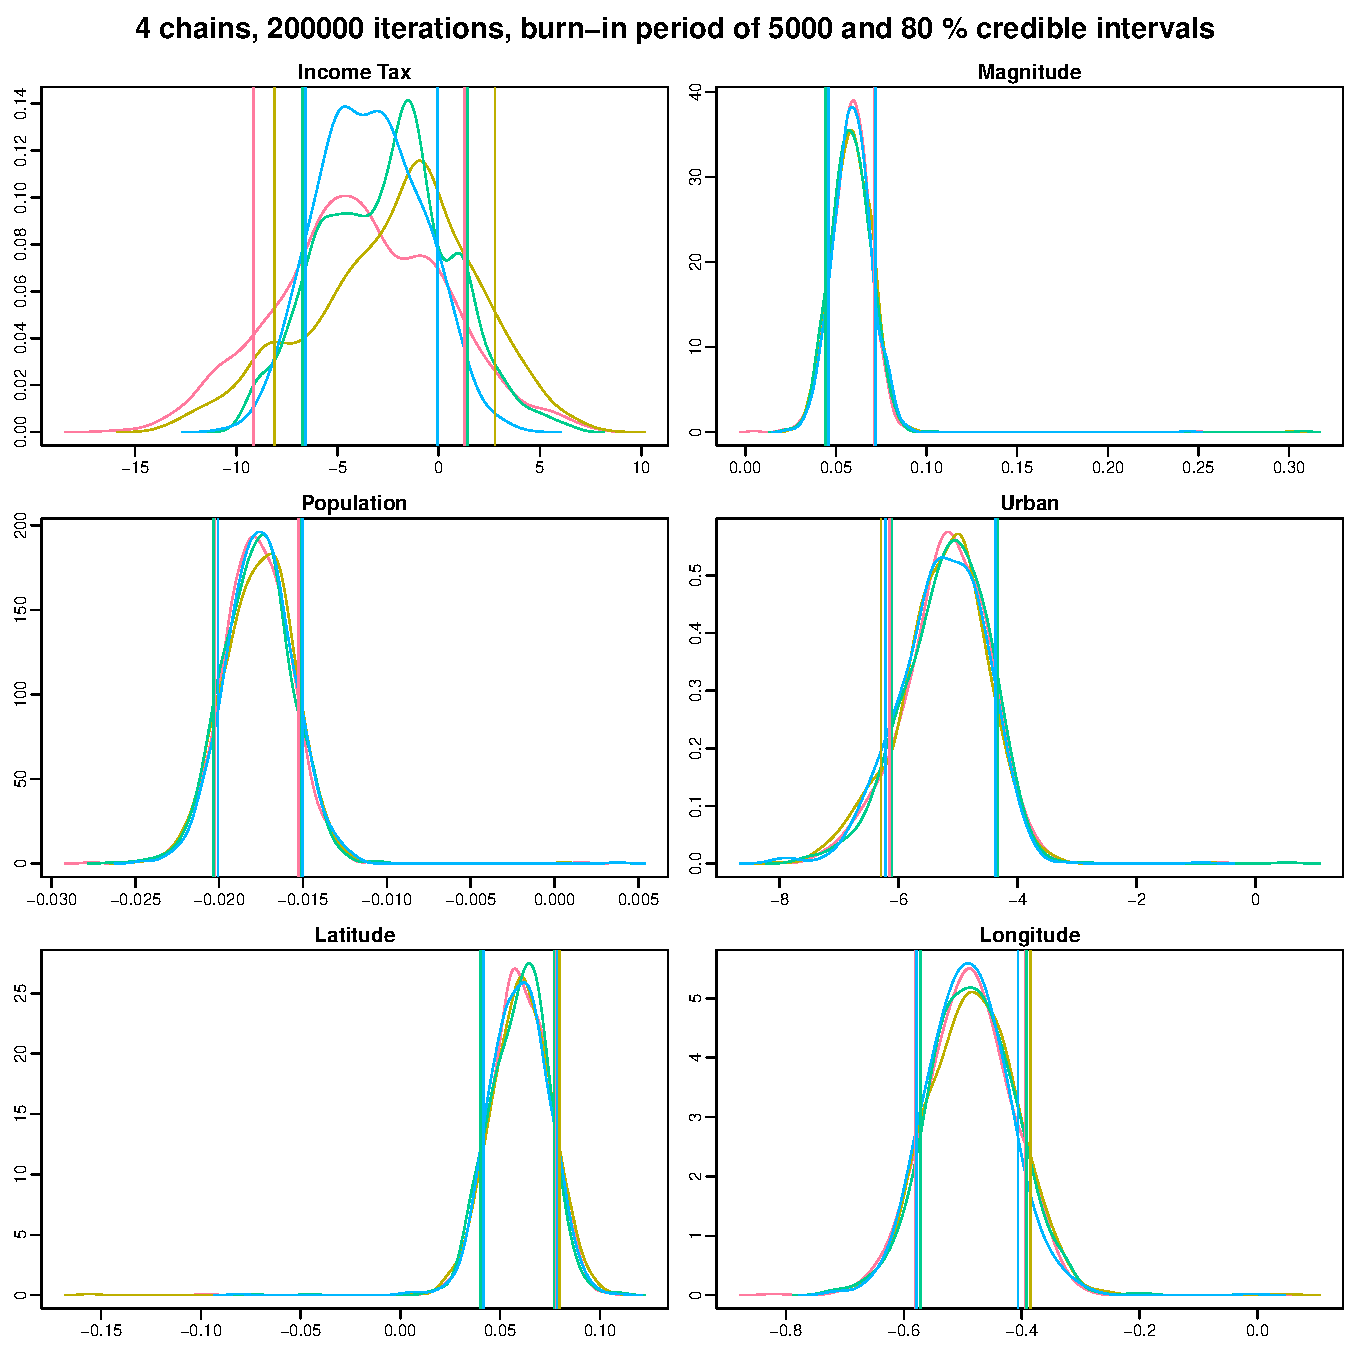
\includegraphics[scale=0.35]{/Users/hectorbahamonde/RU/Dissertation/Papers/Earthquake_Paper/figure/denplot:plot:tax-1.pdf}
\end{frame}
%%%%%%%%%%%%%%%%%%%%%%%%%%%%%%%%%%%%%%%%%%%%%%%%%%%%%%%%%%%%%%%%%%%%%%%%%%





%%%%%%%%%%%%%%%%%%%%%%%%%%%%%%%%%%%%%%%%%%%%%%%%%%%%%%%%%%%%%%%%%%%%%%%%%%
% tax plots: Trace plots
\begin{frame}[label=trace_plot_tax]
%\hspace{-1.16cm} 
\centering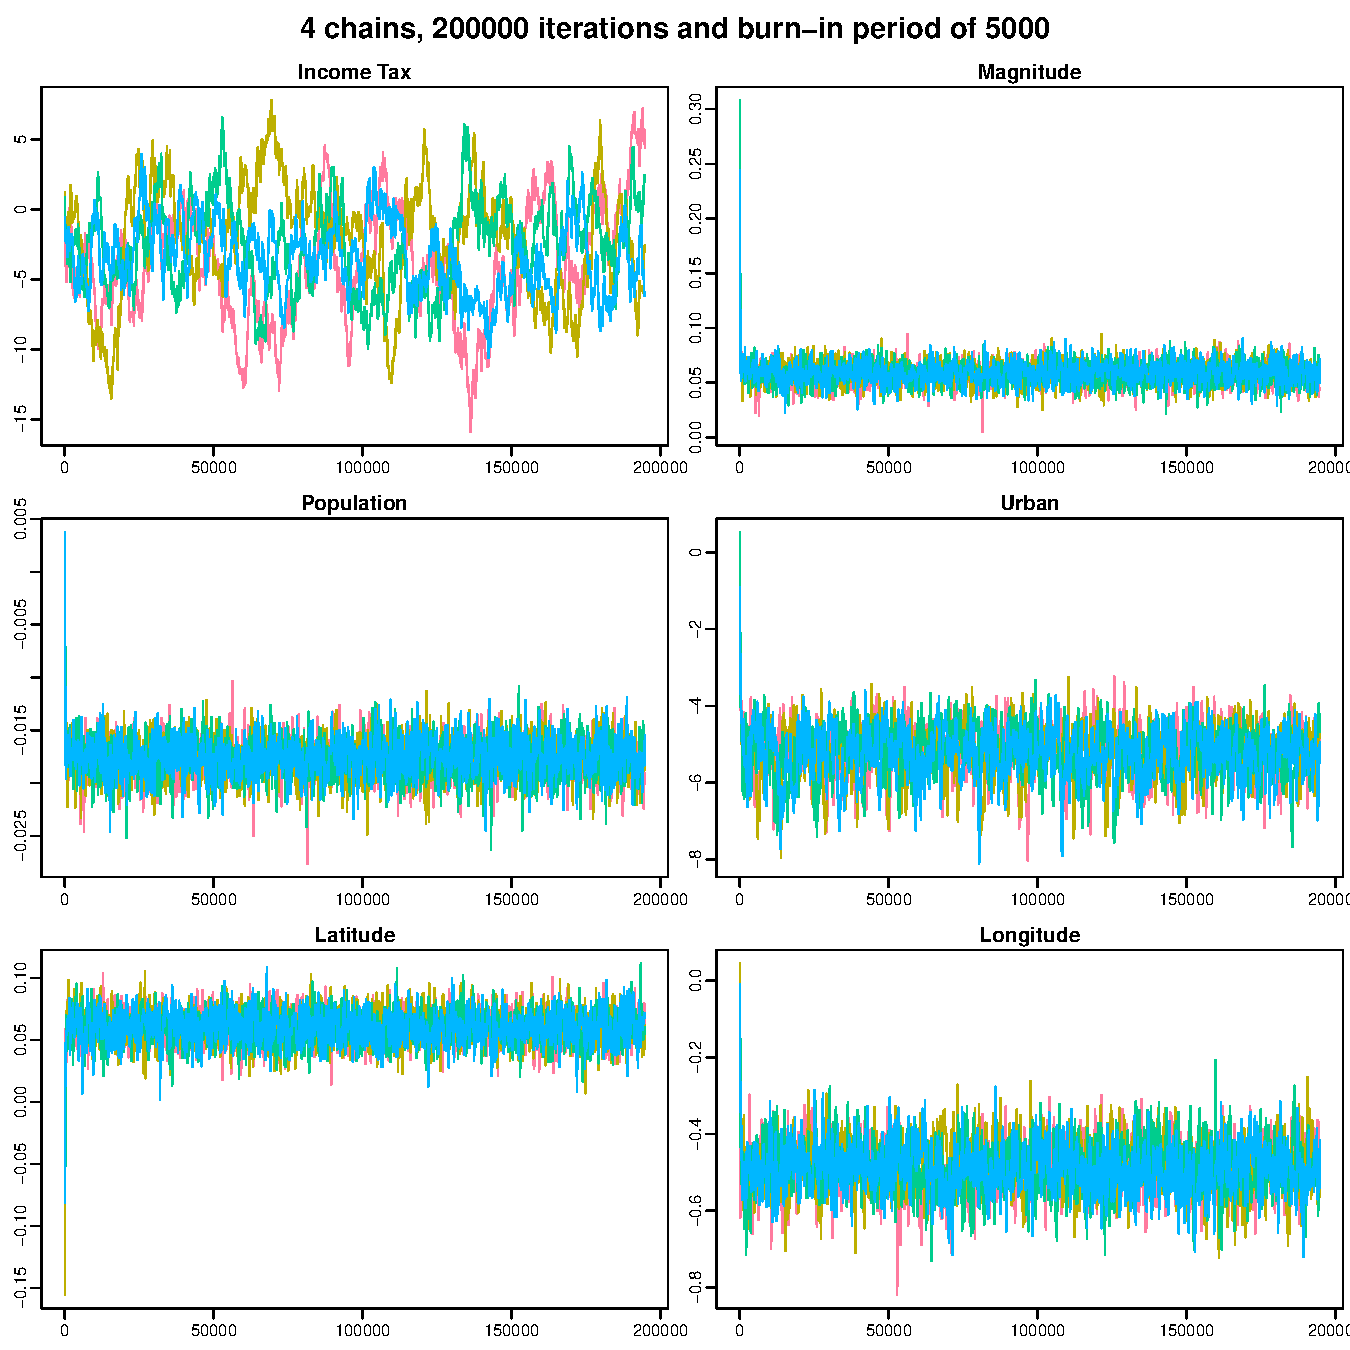
\includegraphics[scale=0.35]{/Users/hectorbahamonde/RU/Dissertation/Papers/Earthquake_Paper/figure/traplot:plot:tax-1}
\end{frame}
%%%%%%%%%%%%%%%%%%%%%%%%%%%%%%%%%%%%%%%%%%%%%%%%%%%%%%%%%%%%%%%%%%%%%%%%%%








%%%%%%%%%%%%%%%%%%%%%%%%%%%%%%%%%%%%%%%%%%%%%%%%%%%%%%%%%%%%%%%%%%%%%%%%%%
% tax model: Reg. Table
\begin{frame}[label=table_tax]
\begin{tabular}{rrrrrr}
  \hline
 & Mean & SD & Lower & Upper & Pr. \\ 
  \hline
Income Tax & -3.01 & 3.55 & -7.55 & 1.41 & 0.81 \\ 
  Magnitude & 0.06 & 0.01 & 0.04 & 0.07 & 1.00 \\ 
  Latitude & 0.06 & 0.01 & 0.04 & 0.08 & 1.00 \\ 
  Longitude & -0.49 & 0.07 & -0.58 & -0.39 & 1.00 \\ 
  Population & -0.02 & 0.00 & -0.02 & -0.02 & 1.00 \\ 
  Urban & -5.22 & 0.73 & -6.19 & -4.35 & 1.00 \\ 
   \hline 
 \multicolumn{6}{l}{ \scriptsize {\bf Note}: 200000 iterations with a burn-in period of n = 5000 iterations discarded.}\\
 \multicolumn{6}{l}{ \scriptsize 80\% credible intervals (upper/lower bounds). All R-Hat statistics below critical levels.}\\
 \multicolumn{6}{l}{ \scriptsize Standard convergence diagnostics suggest good mixing and convergence.}\\
 \multicolumn{6}{l}{ \scriptsize Year fixed effects were omitted in the table.}\\
 \multicolumn{6}{l}{ \scriptsize A total of 4 chains were run. Detailed diagnostic plots available \href{https://github.com/hbahamonde/Earthquake_Paper/raw/master/Bahamonde_Earthquake_Paper_Diagnostic_Plots_Income_Tax_Model.pdf}{\texttt here}.}
 \end{tabular}
\end{frame}
%%%%%%%%%%%%%%%%%%%%%%%%%%%%%%%%%%%%%%%%%%%%%%%%%%%%%%%%%%%%%%%%%%%%%%%%%%



%%%%%%%%%%%%%%%%%%%%%%%%%%%%%%%%%%%%%%%%%%%%%%%%%%%%%%%%%%%%%%%%%%%%%%%%%%
\begin{frame}[label=credible_threats]
For example, the historian Barros (1970) explains that before the civil war, \emph{salitreras} (nitrate towns) in northern Chile were locally so important that they were considered ``a state within the state.'' {\bf Local bosses had to approve decisions on whether public employees could be fired, whether public works could be developed, and on whether politicians could give public speeches}. Moreover, {\color{red}they coined their own currency} and had their own particular {\color{red}local laws}. 
\end{frame}
%%%%%%%%%%%%%%%%%%%%%%%%%%%%%%%%%%%%%%%%%%%%%%%%%%%%%%%%%%%%%%%%%%%%%%%%%%




\end{document}



